\documentclass[letterpaper,final,12pt,reqno]{amsart}

\usepackage[total={6.3in,9.2in},top=1.1in,left=1.1in]{geometry}

\usepackage{times,bm,bbm,empheq,verbatim,fancyvrb,graphicx,amsthm,amssymb}
\usepackage[dvipsnames]{xcolor}
\usepackage{booktabs,multirow,xspace}

\usepackage{tabto}
\TabPositions{1.5cm}

\usepackage{tikz}
\usetikzlibrary{decorations.pathreplacing}
\usetikzlibrary{graphs,quotes}

\usepackage[kw]{pseudo}
\pseudoset{%
left-margin=15mm,%
topsep=5mm,%
label=\footnotesize\arabic*,%
idfont=\texttt,%
ctfont=\textsl,%
ct-left=\qquad\qquad(,%
ct-right=),%
}

\usepackage{float}

% hyperref should be the last package we load
\usepackage[pdftex,
colorlinks=true,
plainpages=false, % only if colorlinks=true
linkcolor=blue,   % ...
citecolor=Red,    % ...
urlcolor=black    % ...
]{hyperref}

\renewcommand{\baselinestretch}{1.05}

\allowdisplaybreaks[1]  % allow display breaks in align environments, if they avoid major underfulls

\newtheoremstyle{cstyle}% name
  {5pt}% space above
  {5pt}% space below
  {\itshape}% body font
  {}% indent amount
  {\itshape}% theorem head font
  {.}% punctuation after theorem head
  {.5em}% space after theorem head
  {\thmname{#1}\thmnumber{ #2}\thmnote{ (#3)}}% theorem head spec
\theoremstyle{cstyle}

\newtheorem{theorem}{Theorem}
\newtheorem{lemma}[theorem]{Lemma}
\newtheorem{corollary}[theorem]{Corollary}
\newtheorem{assumptions}[theorem]{Assumptions}

\newtheoremstyle{cstyle*}% name
  {5pt}% space above
  {5pt}% space below
  {\itshape}% body font
  {}% indent amount
  {\itshape}% theorem head font
  {.}% punctuation after theorem head
  {.5em}% space after theorem head
  {\thmname{#1}}% theorem head spec
\theoremstyle{cstyle*}
\newtheorem{assumptions*}{Assumptions}

\newtheoremstyle{dstyle}% name
  {5pt}% space above
  {5pt}% space below
  {}%{\itshape}% body font
  {}% indent amount
  {\itshape}% theorem head font
  {.}% punctuation after theorem head
  {.5em}% space after theorem head
  {\thmname{#1}\thmnumber{ #2}\thmnote{ (#3)}}% theorem head spec
\theoremstyle{dstyle}

\newtheorem{definition}[theorem]{Definition}
\newtheorem{example}[theorem]{Example}

% numbering
\numberwithin{equation}{section}
\numberwithin{figure}{section}
\numberwithin{table}{section}
\numberwithin{theorem}{section}

\newcommand{\eps}{\epsilon}
\newcommand{\RR}{\mathbb{R}}

\newcommand{\grad}{\nabla}
\newcommand{\Div}{\nabla\cdot}
\newcommand{\trace}{\operatorname{tr}}

\newcommand{\hbn}{\hat{\mathbf{n}}}

\newcommand{\bb}{\mathbf{b}}
\newcommand{\be}{\mathbf{e}}
\newcommand{\bbf}{\mathbf{f}}
\newcommand{\bg}{\mathbf{g}}
\newcommand{\bn}{\mathbf{n}}
\newcommand{\br}{\mathbf{r}}
\newcommand{\bu}{\mathbf{u}}
\newcommand{\bv}{\mathbf{v}}
\newcommand{\bw}{\mathbf{w}}
\newcommand{\bx}{\mathbf{x}}
\newcommand{\by}{\mathbf{y}}
\newcommand{\bz}{\mathbf{z}}

\newcommand{\bF}{\mathbf{F}}
\newcommand{\bV}{\mathbf{V}}
\newcommand{\bX}{\mathbf{X}}

\newcommand{\bxi}{\bm{\xi}}
\newcommand{\bzero}{\bm{0}}

\newcommand{\cK}{\mathcal{K}}
\newcommand{\cV}{\mathcal{V}}

\newcommand{\rhoi}{\rho_{\text{i}}}

\newcommand{\ip}[2]{\left<#1,#2\right>}

\newcommand{\maxR}{R^{\bm{\oplus}}}
\newcommand{\minR}{R^{\bm{\ominus}}}
\newcommand{\iR}{R^{\bullet}}

\newcommand{\nn}{{\text{n}}}
\newcommand{\pp}{{\text{p}}}
\newcommand{\qq}{{\text{q}}}
\newcommand{\rr}{{\text{r}}}

\newcommand{\supp}{\operatorname{supp}}
\newcommand{\Span}{\operatorname{span}}

\newcommand{\fascd}{\pr{fascd}\xspace}

\newcommand{\rNC}{r_{\text{NC}}}
\newcommand{\rSS}{r_{\text{SS}}}
\newcommand{\rXX}{r_{\text{XX}}}

\newcommand{\XX}{{\sffamily X}}


\begin{document}
\title[FAS for nonlinear variational inequalities]{A full approximation storage multilevel method \\ for nonlinear variational inequalities}

\author{Ed Bueler}

\author{Patrick E.~Farrell}

\date{\today}

\begin{abstract}
The \emph{full approximation storage constraint decomposition} (FASCD) multilevel finite element method introduced here is a common extension of the full approximation storage multigrid technique for nonlinear partial differential equations, due to A.~Brandt, and of the constraint decomposition method introduced by X.-C.~Tai for variational inequalities.  We extend the existing constraint decomposition ideas by recognizing and exploiting the telescoping nature of certain function space subset decompositions arising from multilevel mesh hierarchies.  Then, by using strong smoothers with work proportional to the number of unknowns on the finite element mesh level, we demonstrate that FASCD V-cycles show superior mesh-independent convergence rates and that FASCD F-cycles (full multigrid) are optimal solvers.  The example problems include unilateral and bi-obstacle variational inequality problems with linear and nonlinear differential operators.
\end{abstract}

\maketitle

%\tableofcontents

\thispagestyle{empty}
%\bigskip

\newfloat{pseudofloat}{t}{xyz}[section]
\floatname{pseudofloat}{Algorithm}


\section{Introduction} \label{sec:intro}

The constraint decomposition (CD) methods of Tai \cite{Tai2003} are designed to solve coercive variational inequality (VI) problems which arise from minimization of a convex functional over a convex set.  These methods have been shown to converge for multilevel and domain decompositions in a finite element (FE) context.  In the multilevel case, the CD method has been shown to have almost grid-independent error bounds, and near-optimal complexity, for elliptic, linear obstacle problems \cite[Subsection 5.4]{Tai2003}; see also \cite[Theorem 4.6 and Algorithm 4.7]{GraeserKornhuber2009}.  In this paper we extend the multilevel CD method by replacing the coarse-level corrections with a full approximation storage (FAS; \cite{Brandt1977,Bruneetal2015}) approach, and we apply this new solver to nonlinear VI problems which do not arise from minimization.

Specifically, our \emph{full approximation storage constraint decomposition} (FASCD) method extends the algorithms in \cite{GraeserKornhuber2009} and \cite{Tai2003} in the following directions:
\renewcommand{\labelenumi}{\emph{(\roman{enumi})}}
\begin{enumerate}
\item The FAS coarse corrections are adapted for general VI problems.  The needed computations require neither an objective function nor linearity of the residual operator.
\item Box constraints, namely upper and lower obstacles, are permitted; see Section \ref{sec:femultilevel}.
\item We observe an asymmetry special to multilevel CD methods, namely that up-smoothing is more effective than down-smoothing because a ``telescoping'' subset property can be exploited on the up-smoothing side.
\item We implement V-cycles (Algorithm \ref{alg:fascd}) and F-cycles (full multigrid; Algorithm \ref{alg:fascd-fcycle})
\item By using a Newton-type active set method as a smoother, with a fixed number of Krylov iterations per step so that the work of the smoother is proportional to the number of unknowns on the given level, we demonstrate that F-cycle FASCD is an optimal solver.
\end{enumerate}

FASCD V-cycles exhibit essentially the same mesh-independent convergence rates for VI problems that FAS multigrid V-cycles exhibit for the corresponding (unconstrained) PDE problems.  The F-cycle results in Section \ref{sec:results} show nearly-textbook multigrid efficiency, namely solutions within discretization error in work comparable to few smoother sweeps on the finest-level mesh \cite{BrandtLivne2011}, for classical Laplacian obstacle problems, $p$-Laplacian obstacle problems, and nonnegativity-constrained advection-diffusion equations.  Furthermore, these results are essentially insensitive to the length or structure of the free boundary, i.e.~the geometric complexity of the coincidence set.

The iterates from FASCD are admissible, and thus the nonlinear operator in the VI needs only be defined for admissible states.  For example, we solve an ice sheet geometry problem (Examples \ref{ex:sia}, \ref{ex:results:sia}) in which the ice flow formulas are only meaningful for surface elevation iterates which exceed the bed elevation.  (More generally, fluid-layer problems, with a non-negative thickness constraint, often require the solution of an auxiliary PDE on a domain determined inside the VI residual evaluation \cite{Bueler2021conservation}.  However, though a target for future applications of FASCD, such problems are not addressed here.)  Note that non-admissible methods, including semi-smooth methods \cite{BensonMunson2006}, would require unnatural modifications of the operator formula in such a fluid-layer context.  FASCD solves this low-regularity ice sheet problem, wherein the solution has unbounded gradient at the free boundary, by a mesh-independent number of F-cycle iterations.

This paper is organized as follows.  In Section \ref{sec:vi} we recall the theory of coercive and monotone variational inequalities, with several example problems.  Then Section \ref{sec:cd} reviews the basics of CDs, including the associated iterations, as proposed by Tai \cite{Tai2003}.  Section \ref{sec:femultilevel} sets up multilevel FE hierarchies, along with special monotone restriction operators \cite{GraeserKornhuber2009}.  Section \ref{sec:cdmultilevel} presents defect constraints \cite{GraeserKornhuber2009}, leading to an apparently new understanding of telescoping sets for up-smoothing, based on an ``incomplete'' CD.  Section \ref{sec:vcycle} then states the FASCD V-cycle, with Section \ref{sec:implementation} addressing implementation concerns, smoother semantics, and F-cycles.  Section \ref{sec:results} gives FASCD numerical results, for problems in Section \ref{sec:vi}, from a parallel Firedrake \cite{Rathgeberetal2016} implementation.  Discussion and outlook in Section \ref{sec:discussion} and an Appendix, which sketchs how FASCD reduces to classical FAS multigrid for PDEs, finish the work.


\section{Variational inequalities} \label{sec:vi}

Suppose $\cV$ is a real and reflexive Banach space with norm $\|\cdot\|$ and topological dual space $\cV'$.  Denote the dual pairing of $\phi \in \cV'$ and $v\in\cV$ by $\ip{\phi}{v} = \phi(v)$, and define the (Banach space) norm on $\cV'$ by $\|\phi\|_{\cV'} = \sup_{\|v\|=1} |\ip{\phi}{v}|$.  Let $\cK \subset \cV$ be a nonempty, closed, and convex subset, the \emph{constraint set}; elements of $\cK$ are said to be \emph{admissible}.  For a continuous, but generally nonlinear, operator $f:\cK \to \cV'$ and a linear \emph{source functional} $\ell\in \cV'$ we consider the following \emph{variational inequality} (VI) problem, with solution $u^*\in \cK$ if it exists:
\begin{equation}
\ip{f(u^*)}{v-u^*} \ge \ip{\ell}{v-u^*} \qquad \text{for all } v\in \cK. \label{eq:vi}
\end{equation}
Because $f$ is (generally) nonlinear, the source term $\ell$ is not strictly needed in stating this class of problems.  In fact, by redefining $f$ we may take $\ell=0$.  However, allowing $\ell$ clarifies the algorithm in Section \ref{sec:vcycle}.

VI \eqref{eq:vi} generalizes nonlinear systems of equations $f(u^*)=\ell$ to problems where $u^*$ is also constrained to be in $\cK$.  Informally, pretending the dual pairing is an inner product, \eqref{eq:vi} says that the angle between $f(u^*)-\ell$ and any arbitrary vector $v-u^*$ pointing from $u^*$ into $\cK$ is at most $90^\circ$; while $f(u^*)-\ell$ may not be zero, it must point directly into $\cK$.  On the other hand, if $u^*\in\cK^\circ$ is in the interior of the constraint set then \eqref{eq:vi} implies $f(u^*)=\ell$.

The following definitions are standard \cite{KinderlehrerStampacchia1980}.

\begin{definition}  A map $f:\cK \to \cV'$ is \emph{monotone} if
\begin{equation}
\ip{f(u)-f(v)}{u-v} \ge 0 \qquad \text{for all } u,v \in \cK, \label{eq:monotone}
\end{equation}
\emph{strictly monotone} if equality in \eqref{eq:monotone} implies $u=v$, and \emph{coercive} if there exists $w \in \cK$ so that
\begin{equation}
\frac{\ip{f(u)-f(w)}{u-w}}{\|u-w\|} \to +\infty \qquad \text{as } \|u\|\to +\infty. \label{eq:coercive}
\end{equation}
\end{definition}

It is well-known that if $f:\cK \to \cV'$ is continuous, monotone, and coercive then VI \eqref{eq:vi} has a solution \cite[Corollary III.1.8]{KinderlehrerStampacchia1980}, and that the solution is unique when $f$ is strictly monotone.  As is standard in the calculus of variations \cite{Evans2010}, coercivity permits a compactness argument for unbounded sets $\cK$.  (Recall that the closed and bounded subsets of a reflexive Banach space are weakly compact.)  The condition of continuity can be weakened, e.g.~to only apply on finite-dimensional subspaces \cite{KinderlehrerStampacchia1980}, but this is unnecessary in our examples.

Certain of the VIs solved in this paper satisfy a stronger inequality than \eqref{eq:coercive}.

\begin{definition}  Let $p>1$.  The map $f:\cK \to \cV'$ is \emph{$p$-coercive} if there exists $\kappa>0$ such that
\begin{equation}
\ip{f(u)-f(v)}{u-v} \ge \kappa \|u-v\|^p \qquad \text{for all } u,v \in \cK. \label{eq:pcoercive}
\end{equation}
\end{definition}

It is easy to see that if $f$ is $p$-coercive then it is monotone, strictly monotone, and coercive, so the following well-posedness theorem holds.

\begin{theorem}  \label{thm:viwellposed}  If $f:\cK \to \cV'$ is continuous and $p$-coercive then there exists a unique $u^*\in \cK$ solving VI \eqref{eq:vi}.
\end{theorem}

Let $\Omega \subset \RR^d$ denote a bounded, open set with smooth or piecewise-smooth (e.g.~polygonal) boundary.  Sobolev spaces \cite{Evans2010} will be denoted by $W^{k,p}(\Omega)$, for integer $k$ and $1\le p \le \infty$, with $W^{1,p}_0(\Omega)$ denoting the subspace having zero boundary values.

The following example includes the classical and $p$-Laplacian obstacle problems \cite{ChoeLewis1991}.

\begin{example}  \label{ex:plaplacian}  Suppose $p>1$.  For $u,v \in \cV = W^{1,p}_0(\Omega)$ define $f:\cV \to \cV'$ by
\begin{equation}
\ip{f(u)}{v} = \int_\Omega |\grad u|^{p-2} \grad u \cdot \grad v\,dx, \label{eq:plaplacian}
\end{equation}
a continuous map \cite[Theorem A.0.6]{Peral1997}.  For $p\ge 2$, if $x,y\in\RR^d$ then $(|x|^{p-2} x - |y|^{p-2} y)\cdot (x-y) \ge 2^{2-p} |x-y|^p$ \cite[Appendix A]{Bueler2021conservation}, hence it follows from the Poincar\'e inequality that
    $$\ip{f(u) - f(v)}{u-v} \ge 2^{2-p} a_0 \|\grad u - \grad v\|_p^p \ge 2^{2-p} a_0 C \|u-v\|^p$$
for some $C>0$, and thus $f$ is $p$-coercive.  The map \eqref{eq:plaplacian} is also coercive if $1<p<2$, but the proof is somewhat different \cite[Theorem 4.4, for example]{Bueler2021conservation}.  \end{example}

For monotone operators $f$, VI \eqref{eq:vi} generalizes the problem of minimizing a convex function over $\cK$.  In fact, suppose $F:\cK \to \RR$ is lower semi-continuous and (G\^ateau) differentiable with continuous derivative $F':\cK \to \cV'$.  Then $F$ is convex if and only if $F'$ is monotone \cite[Proposition I.5.5]{EkelandTemam1976}.  Furthermore, Proposition II.2.1 in \cite{EkelandTemam1976} shows that if $F$ is convex then \eqref{eq:vi} holds for $f=F'$ if and only if
\begin{equation}
u^* = \operatorname{arg-min}_{v\in\cK} F(v) - \ip{\ell}{v}. \label{eq:minimization}
\end{equation}
The CD methods of Tai \cite{Tai2003} address problem \eqref{eq:minimization}; the analysis in \cite{Tai2003} supposes that an objective $F$ exists with $F'$ 2-coercive.  For Example \ref{ex:plaplacian} we may define
\begin{equation}
F(v) = \frac{1}{p} \int_\Omega |\grad v|^p\,dx. \label{eq:plaplacianobjective}
\end{equation}
Then $F$ is a convex functional and $F'(v) = f(v)$ for $f$ given in \eqref{eq:plaplacian}.  For any closed and convex $\cK\subset \cV$, VI problem \eqref{eq:vi} is then equivalent to optimization problem \eqref{eq:minimization}.

Next we give two examples which are \emph{not} of optimization type \eqref{eq:minimization}, the first being an advection-diffusion problem, which needs the following Lemma.

\begin{lemma}  \label{lem:advectionskew}  \cite{Elmanetal2014}\,  Suppose $\bX :\Omega \to \RR^d$ is a bounded and boundedly-differentiable vector field on $\Omega$ with zero divergence ($\Div \bX=0$).  For $u,v \in W^{1,2}(\Omega)$ let $b(u,v) = \int_\Omega (\bX \cdot \grad u) v\,dx$.  Then $b(u,u) = \frac{1}{2} \int_{\partial \Omega} u^2 \bX\cdot \bn\,dx$ where $\bn$ is the outward normal on $\partial \Omega$.
\end{lemma}

\begin{proof}
Integration by parts gives $b(u,v) = - b(v,u) + \int_{\partial \Omega} uv \bX\cdot \bn\,dx$.
\end{proof}

\begin{example}  \label{ex:advectiondiffusion}  Suppose $\partial\Omega$ is partitioned into Dirichlet and Neumann portions, i.e.~$\partial\Omega = \partial_D\Omega \cup \partial_N\Omega$, with $\partial_D\Omega$ of positive measure.  Let $\cV \subset W^{1,2}(\Omega)$ be the space of functions which are zero along $\partial_D\Omega$.  Consider a divergence-free velocity field $\bX$ on $\Omega$ satisfying the conditions of Lemma \ref{lem:advectionskew}, and assume that the flow is outward on the Neumann boundary: $\bX \cdot \bn \ge 0$ on $\partial_N\Omega$.  For $u,v \in \cV$, $\eps>0$, and $\phi \in L^\infty(\Omega)$, define
\begin{equation}
\ip{f(u)}{v} = \eps \left(\grad u, \grad v\right)_{L^2(\Omega)} + b(u,v) - \ip{\phi}{v}. \label{eq:advectiondiffusion}
\end{equation}
With this operator, consider VI \eqref{eq:vi} for any closed and convex $\cK \subset \cV$ and $g\in\cV'$.  The interior condition, i.e.~PDE strong form, is the following linear advection-diffusion equation
\begin{equation}
-\eps \grad^2 u + \bX\cdot \grad u = \phi.
\label{eq:pdeadvectiondiffusion}
\end{equation}
On the other hand, it is easy to see that $|\ip{f(u)}{v}| \le (\eps + \|\bX\|_\infty + \|\phi\|_\infty) \|u\| \|v\|$, thus that $f:\cK \to \cV'$ is continuous.  Lemma \ref{lem:advectionskew} says that the bilinear form $b(u,v)$ is skew-symmetric up to a nonnegative term.  By the outward flow assumption and the Poincar\'e inequality,
\begin{align*}
\ip{f(u)-f(v)}{u-v} &= \eps \int_\Omega |\grad u - \grad v|^2\,dx + b(u-v,u-v) \\
                    &= \eps \int_\Omega |\grad u - \grad v|^2\,dx + \frac{1}{2} \int_{\partial_N\Omega} (u-v)^2 \bX\cdot\bn \ge \eps C \|u-v\|^2.
\end{align*}
Thus $f$ is 2-coercive, and so VI problem \eqref{eq:vi} is well-posed.
\end{example}

If $\bX \ne 0$ then $f\ne F'$ in Example \ref{ex:advectiondiffusion}, for any objective $F$, because $\ip{f(u)}{v}$ does not possess the symmetry of the gradient of a scalar: for $u,v$ which are zero on $\partial \Omega$, note that $\ip{f(u)}{v} - \ip{f(v)}{u} = -2 b(u,v)$.  References \cite{Bueler2021conservation,ChangNakshatrala2017} consider inequality-constrained advection-diffusion VI problems like this, specifically over the set $\cK = \{v\ge 0\}$.

The next VI example, nonlinear and not of optimization type, is a model for steady ice sheet geometry in a given climate.  Related VI problems arise for any fluid layer which is subject to a source term which can remove the fluid \cite{Bueler2021conservation}.

\begin{example}  \label{ex:sia}  Let $\Omega \subset \RR^2$ be a fixed region of land, and suppose $b \in C^1(\Omega)$ is the given bedrock elevation.  Let $a \in L^\infty(\Omega)$ denote a given ``surface mass balance'' function, the annually-averaged rate of ice accumulation (as snow) minus melt and runoff.  Then the surface elevation $s\in C(\Omega)$ of a steady-state, isothermal, and non-sliding ice sheet (glacier) approximately satisfies the \emph{shallow ice approximation} (SIA) \cite{GreveBlatter2009} problem
\begin{equation}
\int_\Omega \Gamma (s-b)^{n+2} |\grad s|^{n-1} \grad s \cdot \grad (v-s) \,dx \ge \int_\Omega a (v-s)\,dx, \label{eq:siavi}
\end{equation}
over the set $\mathcal{K} = \{s\ge b\}$ of admissible surface elevations, where $n>1$ and $\Gamma>0$ are constants determined by the physical properties of ice; $n=3$ is a typical value.  The doubly-nonlinear and doubly-degenerate operator in this case is
\begin{equation}
\ip{f(s)}{v} = \int_\Omega \Gamma (s-b)^{n+2} |\grad s|^{n-1} \grad s \cdot \grad v\,dx. \label{eq:sia}
\end{equation}
If the bed is flat ($b=0$) then a power transformation converts the problem into $p$-Laplacian form \eqref{eq:plaplacian} with $p=n+1$.  For general beds $b$ less is understood about this operator, but existence holds for \eqref{eq:siavi} \cite{JouvetBueler2012}.  The theory suggests that a power of the solution lives in a Sobolev space, namely $(s-b)^{2p/(p-1)} \in W^{1,p}(\Omega)$.  This theory, and also observations of ice sheets, shows that $|\grad s|$ is generally unbounded as one approaches the free boundary, the \emph{ice margin}, from the icy side (where $s>b$).
\end{example}

Numerical results are shown in Section \ref{sec:results} for applications of FASCD Algorithms \ref{alg:fascd} and \ref{alg:fascd-fcycle} to these Examples.


\section{Constraint decomposition (CD)} \label{sec:cd}

Suppose that there are $m<\infty$ closed subspaces $\cV_i \subset \cV$, so that the sum
\begin{equation}
\cV = \sum_{i=0}^{m-1} \cV_i \label{eq:subspacedecomp}
\end{equation}
holds in the sense that if $w \in \cV$ then there exist $w_i \in \cV_i$ so that $w = \sum_i w_i$.  We say \eqref{eq:subspacedecomp} is a \emph{space decomposition} of $\cV$ \cite{Xu1992}.  For a closed, convex subset $\cK \subset \cV$, suppose further that $\cK_i \subset \cV_i$ are nonempty, closed, and convex subsets such that
\begin{equation}
\cK = \sum_{i=0}^{m-1} \cK_i. \label{eq:constraintdecomp}
\end{equation}
The sum in \eqref{eq:constraintdecomp} must hold in two senses \cite{TaiTseng2002}: \emph{(i)}~if $w \in \cK$ then there exist $w_i \in \cK_i$ so that $w = \sum_i w_i$, and \emph{(ii)}~if $z_i \in \cK_i$ for each $i$ then $\sum_i z_i \in \cK$.  Note that neither decomposition \eqref{eq:subspacedecomp} or \eqref{eq:constraintdecomp} is required to be unique, and also notice that sense \emph{(ii)} is automatic for \eqref{eq:subspacedecomp} because the $\cV_i$ are subspaces.  Finally, suppose there are bounded \emph{decomposition operators}\footnote{Denoted ``$R_i$'' in \cite{Tai2003}.  Here we avoid a notational conflict with multilevel transfer operators (Section \ref{sec:femultilevel}).} $\Pi_i : \cK \to \cK_i$ such that if $v \in \cK$ then
\begin{equation}
v = \sum_{i=0}^{m-1} \Pi_i v.  \label{eq:constraintrestrictionsum}
\end{equation}
The operators $\Pi_i$ are generally nonlinear.  Clearly \eqref{eq:constraintrestrictionsum} implies sense \emph{(i)} for \eqref{eq:constraintdecomp}. Tai \cite{Tai2003} defined a \emph{constraint decomposition} (CD) of $\cK$ to be a choice of $\cV_i,\cK_i,\Pi_i$ satisfying \eqref{eq:subspacedecomp}--\eqref{eq:constraintrestrictionsum}.  Figure \ref{fig:cartoon} suggests how a low-dimensional example might look; note $\cK_i \not\subset \cK$ in this, and in most nontrivial cases as well.

\begin{figure}[ht]
\includegraphics[width=0.6\textwidth]{genfigs/cartoon.pdf}
\caption{A constraint decomposition (CD) for a unilateral obstacle problem on a two-point space $\Omega=\{x_1,x_2\}$, with $\mathcal{V}=\left\{v \,:\, \Omega \to \RR\right\}$ and $\mathcal{K}=\{v\ge \psi\}$.}
\label{fig:cartoon}
\end{figure}

In Sections \ref{sec:femultilevel}--\ref{sec:vcycle} we will introduce multilevel CD discretizations and algorithms for finite-dimensional VI problems.  However, one can observe here that the CD concept applies at the level of the continuum problem, as illustrated in the following two examples, the first of which is an overlapping domain decomposition of a Sobolev space.

\begin{example}  \label{ex:domaindecomposition}  For a bounded domain $\Omega \subset \RR^d$, let $\cV = W_0^{k,p}(\Omega)$ for $k\ge 0$ and $p\ge 1$.  Let $\psi$ be a measurable, real-valued obstacle, defined on $\Omega$, which satisfies $\psi|_{\partial \Omega} \le 0$, and let $\cK = \{v \ge \psi\} \subset \cV$.  Suppose further that $\{\phi_i\}_{i=0}^{m-1}$ is a smooth partition of unity on $\Omega$, satisfying $0 \le \phi_i\le 1$ and $\sum_i \phi_i = 1$, and let $\Omega_i$ be the open support of $\phi_i$.  Let $\cV_i = \{w \in \cV:w|_{\Omega \setminus \Omega_i} =0 \}$, $\cK_i = \{v \in \cV_i: v \ge \phi_i \psi\}$, and $\Pi_i(v) = \phi_i v$.  Then \eqref{eq:subspacedecomp}, \eqref{eq:constraintdecomp}, and \eqref{eq:constraintrestrictionsum} all hold.
\end{example}

Our second example is a disjoint frequency decomposition of a Hilbert space.  A multilevel CD over a finite-dimensional FE discretization, as proposed in Sections \ref{sec:femultilevel}--\ref{sec:cdmultilevel}, approximates such a decomposition.

\begin{example}  \label{ex:frequencydecomposition}  For simplicity suppose $\Omega = (0,a)^d \subset \RR^d$ is a cube, and let $\cV = W_{\text{per}}^{2,k}(\Omega)$ be the periodic functions with square-integrable $k$th derivatives.  Suppose $\psi \in W_{\text{per}}^{2,k}(\Omega)$ and let $\cK = \{v \ge \psi\} \subset \cV$.  Without using any detailed notation for Fourier representation, but noting that the frequencies are discrete because $\Omega$ is compact, suppose $\{\cV_i\}$ are $m<\infty$ subspaces of $\cV$ defined by an (nonoverlapping) partition of $W_{\text{per}}^{2,k}(\Omega)$ by frequency, thus satisfying \eqref{eq:subspacedecomp} as an orthogonal decomposition.  Suppose $P_i:\cV \to \cV_i$ are the corresponding orthogonal projections, satisfying $I = \sum_i P_i$.  Let $\cK_i = \{v \ge P_i \psi\} \subset \cV_i$ and $\Pi_i = P_i$.  Then \eqref{eq:constraintdecomp} and \eqref{eq:constraintrestrictionsum} also hold.
\end{example}

Note that $\cK_i \not\subset \cK$ in these cases; informally speaking, the important inclusion is $\cK_i \subset \cV_i$.

Associated to a constraint decomposition \eqref{eq:subspacedecomp}--\eqref{eq:constraintrestrictionsum} are certain iterative methods \cite{Tai2003,Xu1992}.  Let $0\le \alpha \le 1$ be the \emph{damping parameter}.  Algorithms \ref{alg:basiccd-add} and \ref{alg:basiccd-mult} below, discussed next, solve smaller VI problems over each subset $\cK_i$.  Each Algorithm replaces $u \in \cK$ with a new iterate $w\in\cK$ which should be closer to $u^* \in \cK$ solving \eqref{eq:vi}.

The additive/parallel \pr{cd-add} Algorithm \ref{alg:basiccd-add} generalizes the classical Jacobi iteration.  Here ``\textbf{for all}'' can be computed in any order.  In its VI,
\begin{equation}
\ip{f(u - \Pi_i u + \hat w_i)}{v_i-\hat w_i} \ge \ip{\ell}{v_i-\hat w_i} \qquad \forall v_i \in \mathcal{K}_i, \label{eq:cdaddvi}
\end{equation}
the expression ``$u-\Pi_iu+\hat w_i$'' removes the part of $u$ which lies in $\mathcal{K}_i$, and then adds-back the subset solution $\hat w_i \in \mathcal{K}_i$.

\begin{pseudofloat}[H]
\begin{pseudo*}
\pr{cd-add}(u)\text{:} \\+
    for all $i \in \{0,\dots,m-1\}$: \\+
        \rm{find} $\hat w_i\in \cK_i$ \rm{so that for all} $v_i\in \cK_i$, \\+
            $\ip{f(u - \Pi_i u + \hat w_i)}{v_i-\hat w_i} \ge \ip{\ell}{v_i-\hat w_i}$ \\--
    $\hat w = \sum_i \hat w_i\in\cK$ \\
    return $w=(1-\alpha) u + \alpha \hat w$
\end{pseudo*}
\caption{One additive CD iteration for VI problem \eqref{eq:vi}.}
\label{alg:basiccd-add}
\end{pseudofloat}

The multiplicative/successive \pr{cd-mult} Algorithm \ref{alg:basiccd-mult} generalizes the Gauss-Seidel iteration.  Each subset solution corrects the global iterate immediately, so here the ordering used in the ``\textbf{for}'' loop is important.  In the VI,
\begin{equation}
\ip{f\Big(\sum_{j<i} w_j + \hat w_i + \sum_{j>i} \Pi_j u\Big)}{v_i-\hat w_i} \ge \ip{\ell}{v_i-\hat w_i} \qquad \forall v_i \in \mathcal{K}_i, \label{eq:cdmultvi}
\end{equation}
the sum ``$\sum_{j>i} \Pi_j u$'' should be read as ``those portions of $u$ which have not yet improved''.

\begin{pseudofloat}[H]
\begin{pseudo*}
\pr{cd-mult}(u)\text{:} \\+
    for $i = 0,\dots,m-1$: \\+
        \rm{find} $\hat w_i\in \cK_i$ \rm{so that for all} $v_i\in \cK_i$, \\+
            $\displaystyle \ip{f\Big(\sum_{j<i} w_j + \hat w_i + \sum_{j>i} \Pi_j u\Big)}{v_i-\hat w_i} \ge \ip{\ell}{v_i-\hat w_i}$ \\-
            $w_i = (1-\alpha) \Pi_i u + \alpha \hat w_i\in\cK_i$ \\-
    $\hat w = \sum_i \hat w_i\in\cK$ \\
    return $w=(1-\alpha) u + \alpha \hat w$
\end{pseudo*}
\caption{One multiplicative CD iteration for VI problem \eqref{eq:vi}.}
\label{alg:basiccd-mult}
\end{pseudofloat}

In VIs \eqref{eq:cdaddvi} and \eqref{eq:cdmultvi} the argument of $f$ is an element of $\cK$, as the reader should confirm.

By \eqref{eq:constraintdecomp} and \eqref{eq:constraintrestrictionsum} one may write the test vector $v_i - \hat w_i \in \cV_i$ as a difference of admissible vectors from $\cK$.  For \eqref{eq:cdaddvi} and \eqref{eq:cdmultvi} respectively:
\begin{align}
[u - \Pi_i u + v_i] - [u - \Pi_i u + \hat w_i] &= v_i - \hat w_i, \label{eq:admissibledifferenceadd} \\
\left[\sum_{j<i} w_j + v_i + \sum_{j>i} \Pi_j u\right] - \left[\sum_{j<i} w_j + \hat w_i + \sum_{j>i} \Pi_j u\right] &= v_i - \hat w_i.  \label{eq:admissibledifferencemult}
\end{align}
In this sense the VIs over the subsets $\mathcal{K}_i$ solve the same problem as \eqref{eq:vi}.  Furthermore, let $e_i = \hat w_i - \Pi_i u \in \cV_i$.  The reader may confirm that $\hat w = u + \sum_{i} e_i$ and thus that $w = u + \alpha \sum_i e_i$.  The new iterate $w$ is therefore computed by adding a damped correction from each sub\emph{space} $\mathcal{V}_i$, but in such a manner that $w \in \mathcal{K}$; the corrections preserve admissibility.

We call \pr{cd-add} and \pr{cd-mult} the \emph{basic CD iterations}.  VI problems \eqref{eq:cdaddvi} and \eqref{eq:cdmultvi} are analogous to constrained line searches, and in fact they reduce to such line searches when the $\cV_i$ are one-dimensional.  As shown in the next Lemma, when VI problem \eqref{eq:vi} corresponds to convex optimization \eqref{eq:minimization} then, subject to bounds on the damping $\alpha$, these iterations generate monotonically-decreasing objective values.

\begin{lemma} \cite{Tai2003}  Suppose $f=F'$ for $F:\cK\to\RR$ convex and differentiable, and let $u\in\cK$.  For $0 \le \alpha \le 1$ the output $w \in \cK$ from \pr{cd-mult} satisfies
\begin{equation}
F(w) - \ip{\ell}{w} \le F(u) - \ip{\ell}{u}.  \label{eq:objectivemonotone}
\end{equation}
If $0 \le \alpha \le 1/m$ then \pr{cd-add} likewise satisfies \eqref{eq:objectivemonotone}.
\end{lemma}

\begin{proof}  We assume $\ell=0$ without loss of generality; otherwise define $\tilde F(u)=F(u) - \ip{\ell}{u}$ and observe that the proof goes through for $\tilde F$ essentially unchanged.

To show that each iteration of the \textbf{for} loop in \pr{cd-mult} lowers the objective value, let $z_{i} = \sum_{j\le i} w_j + \sum_{j > i} \Pi_j u \in \cK$, $i=0,\dots,m-1$; this is the state at the end of the $i$th iteration.  Note that $z_{i-1} = \sum_{j < i} w_j + \Pi_i u + \sum_{j > i} \Pi_j u$ for $i>0$.  Therefore by convexity of $F$, observation \eqref{eq:admissibledifferencemult} with $v_i=\Pi_i u$, and \eqref{eq:cdmultvi} we find:
\begin{equation*}
F(z_{i-1}) - F\left(\sum_{j<i} w_j + \hat w_i + \sum_{j > i} \Pi_j u\right) \ge \ip{f\left(\sum_{j<i} w_j + \hat w_i + \sum_{j > i} \Pi_j u\right)}{\Pi_i u - \hat w_i} \ge 0.
\end{equation*}
Using convexity (again) now gives
\begin{align*}
F(z_i) &= F\left((1-\alpha) z_{i-1} + \alpha \left(\sum_{j<i} w_j + \hat w_i + \sum_{j > i} \Pi_j u\right)\right) \\
&\le  (1-\alpha) F(z_{i-1}) + \alpha F\left(\sum_{j<i} w_j + \hat w_i + \sum_{j > i} \Pi_j u\right) \le F(z_{i-1}).
\end{align*}
As $u=z_0$ and $w = z_{m-1}$, the result for \pr{cd-mult} follows.

Suppose $w=u+\alpha\sum_i e_i$ is computed by \pr{cd-add} using $\alpha \le 1/m$.  Considering each $e_i=\hat w_i - \Pi_i u$ separately, convexity of $F$ and VI \eqref{eq:cdaddvi} with $v_i=\Pi_i u$ yields
\begin{equation}
F(u) - F(u+e_i) \ge \ip{f(u+e_i)}{u-(u+e_i)} = \ip{f(u-\Pi_i u + \hat w_i)}{\Pi_i u - \hat w_i} \ge 0. \label{eq:cdaddonereduction}
\end{equation}
Let $v = u+ \frac{1}{m} \sum_i e_i$.  Again using convexity (Jensen's inequality), and \eqref{eq:cdaddonereduction}, we have
\begin{equation*}
F(v) = F\left(\frac{1}{m} \sum_{i=0}^{m-1} (u+e_i)\right) \le \frac{1}{m} \sum_{i=0}^{m-1} F(u+e_i) \le \frac{1}{m} \sum_{i=0}^{m-1} F(u) = F(u).
\end{equation*}
Now define $\lambda = m\alpha$ so $0 \le \lambda \le 1$ and $w = (1-\lambda) u + \lambda v$.  Thus by convexity and the above result, $F(w) \le (1-\lambda) F(u) + \lambda F(v) \le F(u)$.
\end{proof}

When $\alpha=1/m$ then the \pr{cd-add} proof can be simplified because $v=w$ and $\lambda=1$.  In this case $F(w)$ is less than $\frac{1}{m} \sum_i F(u+e_i)$ by Jensen's inequality, which is lower than $F(u)$ by \eqref{eq:cdaddvi} or \eqref{eq:cdmultvi}, which gives inequality \eqref{eq:cdaddonereduction}.

The basic CD iterations are meaningful whether or not we are in the optimization case $f=F'$, and when $f$ is nonlinear, non-local, or defined only on $\cK$.  However, practical and efficient FE implementation for such general operators $f$ seems not to have been addressed in the literature.  References \cite{GraeserKornhuber2009,Tai2003} only apply the CD method to the classical obstacle problem, and which case $f=F'$ is linear, local, and defined for all inputs (on all of $\mathcal{V}$).  Substantial implementation simplifications are available in such cases.

\begin{example}  \label{ex:fnice} Suppose $f:\cV \to \cV'$ is linear and a differential operator, thus local in the sense that for any $z\in\mathcal{V}$ the value $\ip{f(\phi)}{z}$ can be computed by an integral over the support of $\phi$.  Considering \pr{cd-add} for concreteness, by linearity \eqref{eq:cdaddvi} can be rewritten
\begin{equation}
\ip{f(e_i)}{v_i-\hat w_i} \ge \ip{\tilde\ell}{v_i-\hat w_i}, \label{eq:linearlocalvi}
\end{equation}
for all $v_i \in \mathcal{K}_i$, where $\tilde\ell = \ell - f(u)$ incorporates the initial residual $f(u)$.  Note $e_i = \hat w_i - \Pi_i u \in \cV_i$ is not generally admissible---generally $e_i \notin \cK$---but \eqref{eq:linearlocalvi} is meaningful for this $f$.
\end{example}

When $f$ has the locality of Example \ref{ex:fnice}, an FE approximation of VI \eqref{eq:vi} can be solved in any incremental and efficient manner following the techniques in \cite{GraeserKornhuber2009,Tai2003}, namely by computations over hat function supports.\footnote{Compare equations (2.31) and (2.32) in \cite{Farrelletal2021}, which describe the same sense of locality.}  However, for general problems lacking the niceties of Example \ref{ex:fnice}, certain additional ideas are needed for practical implementation of \pr{cd-add} or \pr{cd-mult}.  Section \ref{sec:vcycle} constructs a multiplicative multilevel CD iteration for a general operator $f:\cK\to\cV'$ by applying the full approximation storage (FAS) idea of Brandt \cite{Brandt1977}.

From now on we restrict to the case of \emph{box constraints} \cite{BensonMunson2006,FerrisPang1997}, equivalently \emph{bi-obstacle problems}.  Suppose $\Omega \subset \RR^d$ is open and let $\mathcal{V}=W^{1,p}(\Omega)$.  The \emph{lower obstacle} $\underline{\gamma}$ and the \emph{upper obstacle} $\overline{\gamma}$ are given functions, defined on the closure $\overline{\Omega}$, with values in the extended real line $\tilde\RR = [-\infty,+\infty]$.  Specifically, we suppose $\underline{\gamma} : \overline{\Omega} \to [-\infty,+\infty)$ and $\overline{\gamma} : \overline{\Omega} \to (-\infty,+\infty]$ are measurable, $\underline{\gamma} \le \overline{\gamma}$ on $\overline{\Omega}$, and $\underline{\gamma} \le g_D \le \overline{\gamma}$ on $\partial_D \Omega$.  Also, we assume that $\partial\Omega$ is split into disjoint, measurable sets, $\partial\Omega = \partial_D \Omega \cup \partial_N \Omega$, with $\partial_D \Omega$ of positive measure, to facilitate well-posedness \cite{Evans2010}, and $\partial_N \Omega$ possibly empty.  Dirichlet data\footnote{Dirichlet boundary values are in the trace sense \cite{Evans2010}, and $g_D$ is assumed to be as regular as needed.} $g_D:\partial_D \Omega \to \RR$ then defines
\begin{equation}
\cK = \left\{w\,:\,\underline{\gamma} \le w \le \overline{\gamma} \, \text{ and }\, w\big|_{\partial_D \Omega} = g_D\right\} \subset \cV =W^{1,p}(\Omega), \label{eq:originalconstraintset}
\end{equation}
the closed and convex constraint set.  Note that we are treating inequality and equality (boundary) constraints in a unified manner.

Recalling abstract VI problem \eqref{eq:vi}, we now consider box-constrained cases only, using set \eqref{eq:originalconstraintset}.  Given continuous $f:\cK \to \cV'$, and $\ell \in \cV'$, we will assume that the following is well-posed for $u^*\in \cK$:
\begin{equation}
\ip{f(u^*)}{v-u^*} \ge \ip{\ell}{v-u^*} \qquad \text{for all } v\in \cK. \label{eq:boxdirichletvi}
\end{equation}
Note that $v-u^* \in W_0^{1,p}(\Omega)$, so test functions in \eqref{eq:boxdirichletvi} have zero Dirichlet values.  Any Neumann conditions over $\partial_N \Omega$ are determined by the operator formula for $f$, i.e.~by an integration over $\partial_N\Omega$.  In summary, from now on we consider well-posed VI problems \eqref{eq:boxdirichletvi}, namely box-constrained boundary value problems.


\section{Multilevel finite elements} \label{sec:femultilevel}

We seek to rapidly compute the approximate solution of box-constrained VI problems using finite elements (FE).  Suppose $\Omega \subset \RR^d$ is a (open) bounded polygon.\footnote{Section \ref{sec:results} illustrates $d=1,2,3$ cases.}  We will construct a multilevel FE approximation to problem \eqref{eq:boxdirichletvi} over $\Omega$ using $P_1$ or $Q_1$ elements \cite{Elmanetal2014}, by refining a coarsest mesh into a mesh hierarchy; the goal is an accurate solution on the finest-level mesh.  The hierarchy allows the creation of a multilevel CD of $\cK$, using the ideas in the next two Sections, which permits admissibility-preserving coarse corrections.

The mesh hierarchy and FE spaces can be constructed by standard nested refinement.\footnote{The dimension-dependent details of mesh refinement are suppressed here.  Section \ref{sec:results} only uses $P_1$ elements for intervals, triangles, and tetrahedra, in dimensions $d=1,2,3$ respectively, within the Firedrake framework \cite{Rathgeberetal2016}.}  Suppose $\mathcal{T}^0$ is the \emph{coarsest mesh}, a finite set of non-overlapping, nondegenerate elements with union equal to $\overline{\Omega}$ and maximum edge length (characteristic mesh size) $h_0>0$.  We assume $\mathcal{T}^0$ is conforming, with no hanging nodes.  For $j=1,\dots,J$, let $\mathcal{T}^j$ be the uniform refinement of $\mathcal{T}^{j-1}$ so that each $\mathcal{T}^{j-1}$ element becomes $2^d$ elements in $\mathcal{T}^j$ with maximum edge length $h_j = 2^{-j} h_0$.  We call $J\ge 0$ the \emph{depth} of the hierarchy, $J+1$ the \emph{number of levels}, and $\mathcal{T}^J$ the \emph{finest-level mesh}.  Let $m_j$ be the number of nodes in $\mathcal{T}^j$, so there are $m_j$ \emph{degrees of freedom} at the $j$th level.  Let $\mathcal{V}^j$ be the continuous $P_1$ or $Q_1$ FE space over $\mathcal{T}^j$, with arbitrary boundary values, and observe the following vector space nesting:
\begin{equation}
\mathcal{V}^0 \subset \mathcal{V}^1 \subset \dots \subset \mathcal{V}^J \subset \mathcal{V}=W^{1,p}(\Omega).  \label{eq:fe:nestedspaces}
\end{equation}
On the finest-level mesh let $g_D^J \in \mathcal{V}^J$ satisfy $g_D^J = g_D$ on $\partial_D \Omega$; this restricts $g_D$ in \eqref{eq:originalconstraintset} to be piecewise-linear.

In the VI material which follows, use of higher-order Lagrange elements, i.e.~$P_k$ or $Q_k$ with $k\ge 2$, would imply a ``variational crime'' \cite[Chapter 10]{BrennerScott2007}, special to inequality constraints, which we avoid.  Namely, our FE construction of constraint sets (Section \ref{sec:cdmultilevel}) will require \emph{nodal monotonicity},
\begin{equation}
\bw \ge \bz \quad \implies \quad w \ge z \label{eq:nodalmonotonicity}
\end{equation}
for all $w,z \in \mathcal{V}^j$, where $\bw,\bz \in \RR^{m_j}$ denote vectors of nodal values.  However, for $k\ge 2$ there are hat functions in $P_k$ and $Q_k$, i.e.~functions with nodal values one or zero, which take on negative values \cite[Figure 1.7]{Elmanetal2014}.  Evidently \eqref{eq:nodalmonotonicity} is equivalent to the non-existence of such indefinite-sign hat functions.

To allow box constraints on all meshes in the hierarchy, let $\tilde{\mathcal{V}}^j$ denote the set of functions\footnote{Note that $\tilde{\mathcal{V}}^j$ functions need not be defined everywhere on $\Omega$.} on the nodes of $\mathcal{T}^j$ with values in the extended real line $\tilde{\RR} = [-\infty,+\infty]$.  Suppose that the finest-level \emph{lower} and \emph{upper obstacles} $\underline{\gamma}^J, \overline{\gamma}^J \in \tilde{\mathcal{V}}^J$ satisfy
\begin{equation}
\underline{\gamma}^J \le \overline{\gamma}^J, \qquad \underline{\gamma}^J < +\infty, \qquad -\infty < \overline{\gamma}^J. \label{eq:fe:boxconstraintrequirements}
\end{equation}
Also assume that $\underline{\gamma}^J \le g_D^J \le \overline{\gamma}^J$ on those nodes of $\mathcal{T}^J$ which lie in $\partial_D \Omega$.  Define
\begin{equation}
\mathcal{K}^J = \left\{w\,:\,\underline{\gamma}^J \le w \le \overline{\gamma}^J \text{ on nodes of } \mathcal{T}^J, \, \text{ and } \, w|_{\partial_D\Omega} = g_D^J|_{\partial_D\Omega}\right\} \subset \mathcal{V}^J, \label{eq:fe:fineconstraintset}
\end{equation}
the finest-level \emph{constraint set} of admissible FE functions.  This is a nonempty, closed, and convex subset of $\mathcal{V}^J$.  As $\mathcal{V}^J$ functions never take values $\pm\infty$, inequality in \eqref{eq:fe:fineconstraintset} is strict where $\underline{\gamma}^J, \overline{\gamma}^J$ are infinite; there is no lower or upper constraint, respectively, at such nodes.

Let $f^J:\mathcal{K}^J \to (\mathcal{V}^J)'$ be a discretization of $f$ in \eqref{eq:boxdirichletvi}.  Note that the functional $\ell^J=\ell$ is defined and continuous over $\mathcal{V}^J$.  We seek the FE solution $u^J \in \mathcal{K}^J$ of the finest-level, finite-dimensional, nonlinear VI
\begin{equation}
\ip{f^J(u^J)}{v-u^J} \ge \ip{\ell^J}{v-u^J} \qquad \text{for all } v\in \cK^J. \label{eq:fe:vi}
\end{equation}
If $f^J$ is continuous and $p$-coercive on $\mathcal{K}^J$, in the sense that \eqref{eq:pcoercive} holds for all $u,v \in \mathcal{K}^J$, then, as for \eqref{eq:vi}, FE VI \eqref{eq:fe:vi} is well-posed.

While \eqref{eq:fe:vi} approximates \eqref{eq:boxdirichletvi}, we warn the reader that it may not technically be conforming for that VI.  That is, even if quadrature and other implementation details for $f^J$ are ignored, and despite the vector space inclusion $\mathcal{V}^J \subset \mathcal{V}$, we do not require or generally expect $\mathcal{K}^J \subset \mathcal{K}$.  Regardless of the smoothness of the continuum obstacles $\underline{\gamma}, \overline{\gamma}$, admissibility with respect to their FE interpolants $\underline{\gamma}^J, \overline{\gamma}^J$ will generally not imply continuum admissiblity.\footnote{This caveat is especially relevant in geophysical situations where only nodal values of the obstacle are known.  The nodal elevation data misses the actual topographic detail in-between the nodes.  See the Greenland ice sheet application in \cite{Bueler2016}, for example.}

The multilevel algorithm defined in the next two Sections, a solver for FE VI \eqref{eq:fe:vi}, requires transfer operators between meshes.  We require five such operators, of which three are standard multigrid tools \cite{Trottenbergetal2001}.  Table \ref{tab:transfers} will help the reader keep track.

\begin{table}[H]
\begin{tabular}{llc}
\emph{name}  & \emph{action}  & \emph{linear?} \\ \hline
canonical prolongation        & $P:\mathcal{V}^{j-1}\to\mathcal{V}^j$ & \,\checkmark \\
canonical (dual) restriction  & $R:(\mathcal{V}^j)'\to(\mathcal{V}^{j-1})'$ & \,\checkmark \\
(nodal) injection             & $\iR:\mathcal{V}^j\to\mathcal{V}^{j-1}$ & \,\checkmark \\
maximum restriction           & $\maxR:\tilde{\mathcal{V}}^j\to\tilde{\mathcal{V}}^{j-1}$ & \\
minimum restriction           & $\minR:\tilde{\mathcal{V}}^j\to\tilde{\mathcal{V}}^{j-1}$ &
\end{tabular}

\medskip
\caption{Transfer operators used in this paper.}
\label{tab:transfers}
\end{table}

Canonical prolongation $P:\mathcal{V}^{j-1}\to\mathcal{V}^j$ is the vector space inclusion $\mathcal{V}^{j-1} \hookrightarrow \mathcal{V}^j$ of coarser-mesh functions.  Canonical (dual) restriction $R:(\mathcal{V}^j)'\to(\mathcal{V}^{j-1})'$ also acts as an identity in the sense that if $\sigma \in (\mathcal{V}^j)'$ then $(R\sigma)[z] = \sigma[z]$ for all $z \in \mathcal{V}^{j-1} \subset \mathcal{V}^j$.  Note that these canonical transfers generally involve a change of FE representation.  For example, the formula for canonical restriction, derived by writing coarser-mesh hat functions in terms of finer-mesh ones, is ``full-weighting'' \cite{Trottenbergetal2001}.

To define injection $\iR:\mathcal{V}^j\to\mathcal{V}^{j-1}$, observe that the nodes of $\mathcal{T}^{j-1}$ are nodes of $\mathcal{T}^j$, and that for any values at $\mathcal{T}^j$ nodes there is a unique $\mathcal{V}^j$ function assuming those values.  For $z\in\mathcal{V}^j$ we define the injection $\iR z$ as the element of $\mathcal{V}^{j-1}$ with the same (coarse) nodal values.  Note that injection is monotonic: if $w \le z$ then $\iR w \le \iR z$.

Finally, the monotone restrictions \cite{GraeserKornhuber2009} $\maxR,\minR$ are nonlinear maps which maximize and minimize, respectively, nodal values over the open supports of coarser-mesh hat functions.  These monotone operators will only be applied to nodal functions $\tilde{\mathcal{V}}^j$.  To make the definitions precise, let $x_q^j$, $q=0,1,\dots,m_j-1$, denote the nodes of mesh $\mathcal{T}^j$, and denote the corresponding hat functions by $\psi_q^j(x)$.  The monotone restrictions of an $\tilde\RR$-valued\footnote{In computing $\max$ and $\min$ to define \eqref{eq:fe:monotonerestrictions}, the usual $\tilde\RR$ ordering is applied.} nodal function $z\in\tilde{\mathcal{V}}^j$ are the following functions in $\tilde{\mathcal{V}}^{j-1}$:
\begin{align}
(\maxR z)(x_p^{j-1}) &= \max \{z(x_q^j) \,:\, \psi_p^{j-1}(x_q^j) > 0\}, \label{eq:fe:monotonerestrictions} \\
(\minR z)(x_p^{j-1}) &= \min \{z(x_q^j) \,:\, \psi_p^{j-1}(x_q^j) > 0\}, \notag
\end{align}
for $p=0,1,\dots,m_{j-1}-1$.  By standard nested refinement, a coarse-mesh node $x_p^{j-1}$ is in the set of fine nodes $x_q^j$ such that $\psi_p^{j-1}(x_q^j)>0$, so it follows that
\begin{equation}
\minR z \le z \le \maxR z,  \label{eq:fe:monotonerestrictionprops}
\end{equation}
On the other hand, $z\ge 0$ implies $\minR z \ge 0$ and $z \le 0$ implies $\maxR z \le 0$.  These ordering properties used in the CD construction of the next two sections.


\section{Multilevel CDs from level defect constraints} \label{sec:cdmultilevel}

Our practical multilevel CD scheme in this Section uses \emph{defect constraints} \cite{GraeserKornhuber2009} which are based on an admissible finest-level iterate.  The next Example concretely illustrates why we do not apply restriction operators directly to the finest-level box constraints $\underline{\gamma}^J,\overline{\gamma}^J$ in definition \eqref{eq:fe:fineconstraintset}.  Our straightforward iterate-dependent bounds, namely defect constraints \eqref{eq:fe:defectconstraints} below, bypass the difficulties exposed in Example \ref{ex:directRbad}.  However, other successful schemes may exist.

\begin{example}  \label{ex:directRbad}  
For concreteness, suppose $\Omega = [0,L] \subset \RR^1$ is an interval and consider a two-level mesh hierarchy ($J=1$).  Let $\underline{\gamma}^1$ be a sawtooth function with minimum value zero, and suppose $\overline{\gamma}^1=C+\underline{\gamma}^1$ with $C>0$ which is strictly less than the range of $\underline{\gamma}^1$.  Supposing empty Dirichlet boundary for simplicity, the constraint set $\mathcal{K}^1$ defined by \eqref{eq:fe:fineconstraintset} is nonempty.  Figure \ref{fig:directRbad} shows such functions; here levels $\mathcal{T}^1$ and $\mathcal{T}^0$ have $5$ and $3$ nodes, respectively.  However, various restriction schemes applied directly to $\underline{\gamma}^1,\overline{\gamma}^1$ are problematical.  Suppose we propose
    $$\underline{\gamma}^0, \overline{\gamma}^0 \equiv \iR \underline{\gamma}^1, \iR \overline{\gamma}^1. \qquad \text{\emph{[problematic]}}$$
Then $\underline{\gamma}^0=0$ and $\overline{\gamma}^0=C$ identically.  In that case the corresponding constraint set $\mathcal{K}^0$ is nonempty, but prolongation $Pw^0$ of an admissible solution of the coarse problem ($\underline{\gamma}^0 \le w^0 \le \overline{\gamma}^0$) is not admissible on the finer level: $Pw^0 \notin \mathcal{K}^1$.  On the other hand, suppose we propose
    $$\underline{\gamma}^0, \overline{\gamma}^0 \equiv \maxR \underline{\gamma}^1, \minR \overline{\gamma}^1. \qquad \text{\emph{[problematic]}}$$
The general motivation for this choice---compare \eqref{eq:fe:chilevels}---is that $w^0 \ge \underline{\gamma}^0 \, \implies \, Pw^0 \ge \underline{\gamma}^1$ and $w^0 \le \overline{\gamma}^0 \, \implies \, Pw^0 \le \overline{\gamma}^1$.  However, while these facts are true, the difficulty should be clear: the coarse-level admissible set $\mathcal{K}^0$ is now empty because the proposed lower bound $\underline{\gamma}^0$ actually exceeds the proposed upper bound $\overline{\gamma}^0$.
\end{example}

\begin{figure}[ht]
\begin{center}
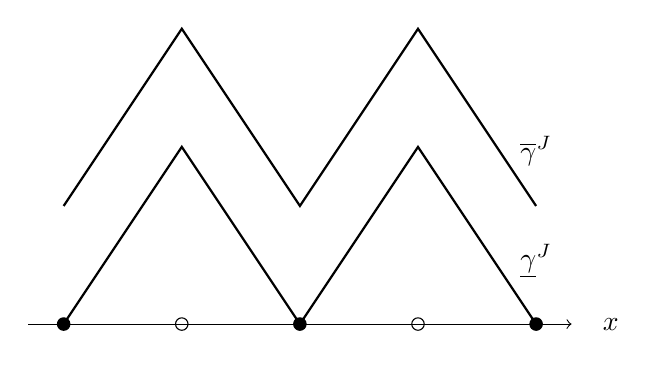
\begin{tikzpicture}[scale=1.5]
  \draw[black,thick] (0.0,0.0) -- (1.0,1.5) -- (2.0,0.0) -- (3.0,1.5) -- (4.0,0.0)
                     node [yshift=8mm] {$\underline{\gamma}^J$};
  \draw[black,thick] (0.0,1.0) -- (1.0,2.5) -- (2.0,1.0) -- (3.0,2.5) -- (4.0,1.0)
                     node [yshift=7mm] {$\overline{\gamma}^J$};
  \draw[black,thin,->] (-0.3,0.0) -- (4.3,0.0) node [xshift=5mm] {$x$};
  \filldraw (0.0,0.0) circle (1.5pt) (2.0,0.0) circle (1.5pt) (4.0,0.0) circle (1.5pt);
  \draw (1.0,0.0) circle (1.5pt) (3.0,0.0) circle (1.5pt);
  %\draw     (5*\hstep,3*\vstep) node[xshift=11mm] {$z_3 \in \mathcal{U}^3$} circle (2.5pt);
\end{tikzpicture}

\end{center}
\caption{For finest-level box constraints $\underline{\gamma}^1,\overline{\gamma}^1$ like these, direct restriction using any of $\iR,\minR,\maxR$, to a coarser mesh (solid dots), is problematic for admissibility of coarse corrections.}
\label{fig:directRbad}
\end{figure}

Subtraction of an admissible iterate provides a route out of these difficulties.  Suppose $w^J \in \cK^J$ is an admissible finest-level iterate (i.e.~which approximates the solution $u^J$ of \eqref{eq:fe:vi}).  We define the \emph{finest-level defect constraints} (DCs) \cite{GraeserKornhuber2009} as the following nodal functions in $\tilde{\mathcal{V}}^J$:
\begin{equation}
\underline{\chi}^J = \underline{\gamma}^J - w^J, \qquad \overline{\chi}^J = \overline{\gamma}^J - w^J. \label{eq:fe:defectconstraints}
\end{equation}
Definition \eqref{eq:fe:fineconstraintset} implies that $\underline{\chi}^J \le 0 \le \overline{\chi}^J$ everywhere in $\overline{\Omega}$, including along the Dirichlet boundary $\partial_D\Omega$.  If $\underline{\gamma}^J=-\infty$ then $\underline{\chi}^J=-\infty$ by definition, and similarly if $\overline{\gamma}^J=+\infty$ then $\overline{\chi}^J=+\infty$.  Observe that a corrected iterate $w^J + z^J$ is admissible, $w^J + z^J \in \cK^J$, if and only if the perturbation $z^J$ is zero on $\partial_D\Omega$ and it is bounded by the defect constraints, $\underline{\chi}^J \le z^J \le \overline{\chi}^J$.

Descending coarser levels, $j=J-1,\dots,1,0$, we apply the monotone restrictions to generate box \emph{level defect constraints} (LDCs) in $\tilde{\mathcal{V}}^j$:
\begin{equation}
\underline{\chi}^{j} = \maxR \underline{\chi}^{j+1}, \qquad \overline{\chi}^{j} = \minR \overline{\chi}^{j+1}. \label{eq:fe:chilevels}
\end{equation}
Observe that
\begin{equation}
\underline{\chi}^{J} \le \dots \le \underline{\chi}^0 \le 0 \le \overline{\chi}^0 \le \dots \le \overline{\chi}^J. \label{eq:fe:chiordering}
\end{equation}
A unilateral $J=4$ example of LDCs $\underline{\chi}^j$ is shown in Figure \ref{fig:chiphilevels}.  The LDC $\underline{\chi}^j$ is the most-negative function from $\tilde{\mathcal{V}}^j$ such that if another element of $\tilde{\mathcal{V}}^j$ is above $\underline{\chi}^j$ then it is also above $\underline{\chi}^{j+1}$, and similar comments apply to $\overline{\chi}^{j}$.

%REGENERATE using https://github.com/bueler/mg-glaciers:
%$ cd mg-glaciers/py/
%$ [modify decomposition() inside visualize.py to turn off axes and print \gamma for obstacle]
%$ ./obstacle.py -J 5 -jcoarse 1 -random -randommodes 8 -diagnostics -o defect.pdf
%fine level 5 (m=63): using 20 V(1,0) cycles -> 38.750 WU
\begin{figure}[ht]
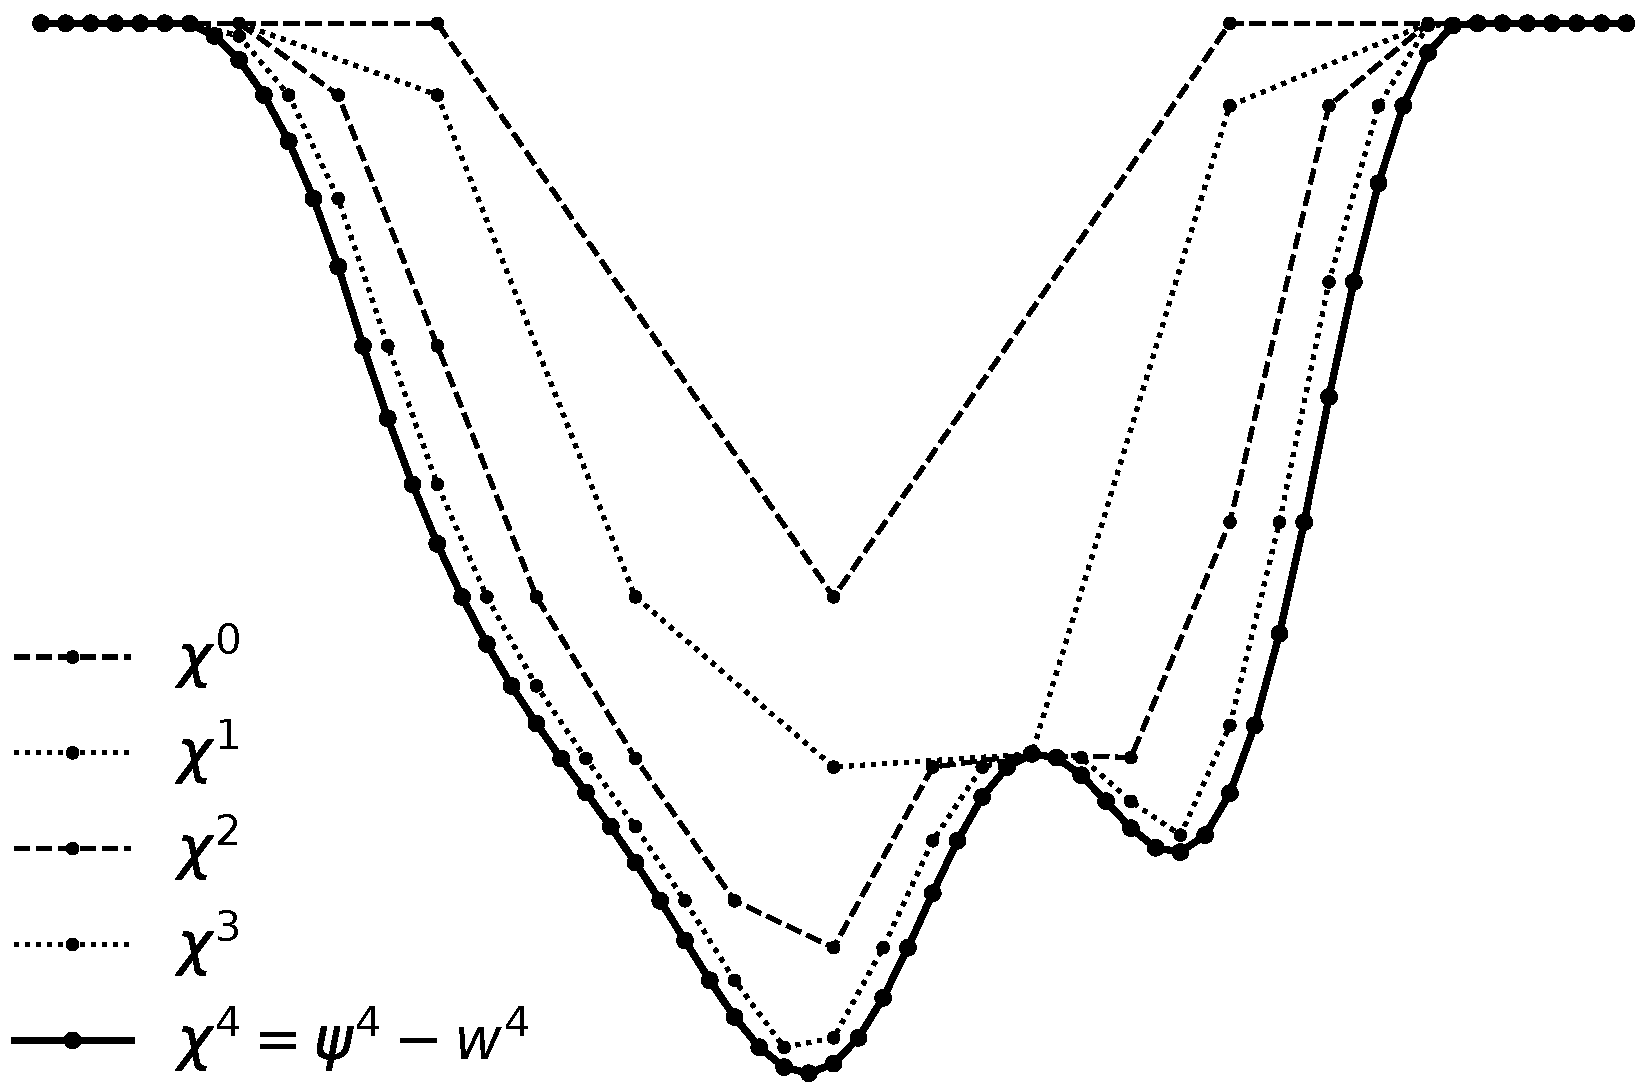
\includegraphics[width=0.65\textwidth]{fixfigs/chiphilevels.pdf}
\caption{Unilateral LDCs $\underline{\chi}^j$ are generated from $\underline{\chi}^J = \underline{\gamma}^J - w^J$ using maximum restriction: $\underline{\chi}^j = \maxR \underline{\chi}^{j+1}$.}
\label{fig:chiphilevels}
\end{figure}

This construction of multilevel box constraints is designed to permit the largest admissible coarse corrections, which promotes multilevel solver efficiency.  Note that for the multilevel schemes in Sections \ref{sec:vcycle} and \ref{sec:implementation}, any system satisfying \eqref{eq:fe:chiordering} will suffice; the particular formulas in \eqref{eq:fe:chilevels} are actually not required.  Also, though the system here is fundamentally the same as the unilateral defect constraints in \cite{GraeserKornhuber2009}, a system for box defect constraints has not been found in the literature.

We now compute the LDC differences (compare \cite{GraeserKornhuber2009}):
\begin{equation}
\underline{\phi}^j = \underline{\chi}^j - \underline{\chi}^{j-1}, \qquad \overline{\phi}^j = \overline{\chi}^j - \overline{\chi}^{j-1}.  \label{eq:fe:philevels}
\end{equation}
We take $\underline{\chi}^{-1}=\overline{\chi}^{-1}=0$ so that $\underline{\phi}^0=\underline{\chi}^0$ and $\overline{\phi}^0=\overline{\chi}^0$.  Regarding subtraction of extended real-valued quantities, if $\underline{\chi}^j(x_p)=-\infty$ then we set $\underline{\phi}^j(x_p)=-\infty$ regardless of the value of $\underline{\chi}^{j-1}(x_p)$, and similarly $\overline{\phi}^j(x_p)=+\infty$ if $\overline{\chi}^j(x_p)=+\infty$.  These new LDCs $\underline{\phi}^{j},\overline{\phi}^{j} \in \tilde{\mathcal{V}}^J$ again bracket zero, $\underline{\phi}^j \le 0 \le \overline{\phi}^j$, but they are not ordered as in \eqref{eq:fe:chiordering}.  Table \ref{tab:ldcs} should help the reader keep track of our box-constrained LDC system.

\begin{table}[H]
\begin{tabular}{lll}
\emph{name}         & \emph{formulas} & \emph{indices} \\ \hline
finest-level DCs & ${\Large \strut} \underline{\chi}^J = \underline{\gamma}^J - w^J,\, \overline{\chi}^J = \overline{\gamma}^J - w^J$ \\
upward LDCs  & ${\Large \strut} \underline{\chi}^{j} = \maxR \underline{\chi}^{j+1}, \, \overline{\chi}^{j} = \minR \overline{\chi}^{j+1}$ & $j=0,\dots,J-1$ \\
downward LDCs       & ${\Large \strut} \underline{\phi}^j = \underline{\chi}^j - \underline{\chi}^{j-1}, \, \overline{\phi}^j = \overline{\chi}^j - \overline{\chi}^{j-1}$ & $j=0,\dots,J$
\end{tabular}

\medskip
\caption{Level defect constraints (LDCs) for box-constrained VI problems.}
\label{tab:ldcs}
\end{table}

The corresponding \emph{downward/upward constraint sets}, respectively, are
\begin{align}
\mathcal{D}^j = \left\{v \in \mathcal{V}^j \,:\, \underline{\phi}^j \le v \le \overline{\phi}^j \text{ and } \, v|_{\partial_D\Omega} = 0\right\}, \label{eq:fe:constraintsets} \\
\mathcal{U}^j = \left\{v \in \mathcal{V}^j \,:\, \underline{\chi}^j \le v \le \overline{\chi}^j \text{ and } \, v|_{\partial_D\Omega} = 0\right\}. \notag
\end{align}
These are closed and convex subsets of the FE spaces $\mathcal{V}^j$.  Because $\underline{\chi}^j \le \underline{\phi}^j \le 0 \le \overline{\phi}^j \le \overline{\chi}^j$, it follows that $\mathcal{D}^j \subseteq \mathcal{U}^j$.  Note that the finest-level set $\mathcal{U}^J$ is equivalent to the original constraint set $\mathcal{K}^J$: for all $z^J \in \mathcal{V}^J$,
\begin{equation}
z^J \in \mathcal{U}^J \quad \iff \quad w^J+z^J \in \mathcal{K}^J. \label{eq:fe:finestlevelequivalent}
\end{equation}

The multilevel V-cycle solver defined in the next Section computes coarse corrections in $\mathcal{D}^j$ for the downward side and in $\mathcal{U}^j$ for the upward side.  Our multilevel strategy is, however, based on \emph{incomplete} CDs (Section \ref{sec:cd}), in the general box-constrained cases, as we now explain.  Each upward set $\mathcal{U}^j$ can be decomposed in an inclusion sense, becoming a true CD in unilateral cases.  The following Lemma is based in part on the unilateral CD construction underlying Algorithm 4.7 in \cite{GraeserKornhuber2009}; see also equation (59) in \cite{Tai2003}.

\begin{lemma}  \label{lem:downwardadmissibility}  For arbitrary finest-level box constraints $\underline{\gamma}^J,\overline{\gamma}^J$ satisfying \eqref{eq:fe:boxconstraintrequirements}, it follows that
\begin{equation}
\mathcal{U}^j \supseteq \mathcal{D}^j + \mathcal{D}^{j-1} + \dots + \mathcal{D}^0 \label{eq:fe:downwardsuminclusion}
\end{equation}
for $j=0,1,\dots,J$.  In unilateral cases, where either $\underline{\gamma}^J=-\infty$ identically or $\overline{\gamma}^J=+\infty$ identically, inclusion \eqref{eq:fe:downwardsuminclusion} becomes a full CD \eqref{eq:subspacedecomp}--\eqref{eq:constraintrestrictionsum} with $\mathcal{U}^j=\sum_{i=0}^j \mathcal{D}^i$.
\end{lemma}

\begin{proof}  Subspace decomposition \eqref{eq:subspacedecomp} holds---see nesting \eqref{eq:fe:nestedspaces}---and definition \eqref{eq:fe:constraintsets} shows $\mathcal{D}^i \subset \mathcal{U}^i \subset \cV^i$.  Furthermore, telescoping sums hold for any $j=0,1,\dots,J$:
\begin{equation}
\sum_{i=0}^j \underline{\phi}^i = \underline{\chi}^j, \qquad \sum_{i=0}^j \overline{\phi}^i = \overline{\chi}^j.  \label{eq:fe:telescoping}
\end{equation}
Thus if $y^i \in \mathcal{D}^i$ for $0 \le i \le j$ then
\begin{equation}
\underline{\chi}^j = \sum_{i=0}^j \underline{\phi}^i \le \sum_{i=0}^j y^i \le \sum_{i=0}^j \overline{\phi}^i \le \overline{\chi}^j, \label{eq:fe:lemmaordering}
\end{equation}
so \eqref{eq:fe:downwardsuminclusion} holds for any box constraints.

In unilateral cases we can also construct decomposition operators $\Pi_i$ and thereby show property \eqref{eq:constraintrestrictionsum}.  For concreteness suppose $\overline{\gamma}^J=+\infty$, thus $\overline{\chi}^j=+\infty$ and $\overline{\phi}^i = +\infty$ for all levels.  For $v\in \mathcal{V}^j$ and $0\le i \le j$, let $I_{j\to i}^\ominus$ be the operator applying the minimum (monotone) restriction $j-i$ times, mapping into $\mathcal{V}^i$:
\begin{equation}
I_{j\to i}^\ominus v = \minR(\dots(\minR v)\dots)  \label{eq:fe:minimummaps}
\end{equation}
Note that $I_{j\to j}^\ominus v = v$, and set $I_{j\to -1}^\ominus=0$ by definition.  From operators \eqref{eq:fe:minimummaps} we define the following nonlinear decomposition operators $\Pi_i:\mathcal{U}^j \to \mathcal{D}^i$:
\begin{equation}
\Pi_i z^j = I_{j\to i}^\ominus(z^j - \underline{\chi}^j) - I_{j\to i-1}^\ominus(z^j - \underline{\chi}^j) + \underline{\phi}^i.  \label{eq:fe:unilateraldecompositionoperator}
\end{equation}
(Compare equation (4.9) in \cite{GraeserKornhuber2009}.)  Property \eqref{eq:fe:monotonerestrictionprops} implies $I_{j\to i}^\ominus(z^j - \underline{\chi}^j) \ge I_{j\to i-1}^\ominus(z^j - \underline{\chi}^j)$, thus $\Pi_i z^j \ge \underline{\phi}^i$, so $\Pi_i z^j \in \mathcal{D}^i$ (in this unilateral case).  On the other hand, the following sum telescopes, leaving only its first term plus the sum in \eqref{eq:fe:telescoping}:
\begin{align*}
\sum_{i=0}^j \Pi_i z^j &= z^j - \underline{\chi}^j + \sum_{i=0}^j \underline{\phi}^i = z^j.
\end{align*}
This shows \eqref{eq:constraintrestrictionsum}, thus that \eqref{eq:fe:downwardsuminclusion} is equality, yielding a true CD \eqref{eq:constraintdecomp}.

The $\underline{\gamma}^J=-\infty$ case is similar.
\end{proof}

One might try to turn \eqref{eq:fe:downwardsuminclusion} into a full CD for arbitrary box constraints by using decomposition maps like $\Pi_i$, for example by splitting $z^j = \min\{z^j,0\} + \max\{z^j,0\}$ and applying unilateral formulas like \eqref{eq:fe:unilateraldecompositionoperator} to $\min\{z^j,0\}$ and $\max\{z^j,0\}$ separately.  In fact, the lower bound $\Pi_i (\min\{z^j,0\}) \ge \underline{\phi}^i$ holds, as shown in the above proof.  However, the following Example shows why $\Pi_i(\min\{z^j,0\})$ may have an arbitrarily large maximum, and thus exceed any finite upper LDC $\overline{\phi}^i$.  In fact, $\Pi_i$ does not generally map all non-positive elements of $\mathcal{U}^J$ into $\mathcal{D}^i$ if a finite upper LDC is present.  Note that this Example does not exclude the existence of an entirely-different strategy for showing a full CD in the general box-constrained case.

\begin{example}  \label{ex:notfullcd}
Let $a\ge 0$ be an arbitrary positive number.  Consider a 2-level hierarchy ($J=1$), and suppose the lower defect constraint is the constant function $\underline{\chi}^1=-a$.  Recalling Table \ref{tab:ldcs}, note $\underline{\chi}^0=\maxR \underline{\chi}^1=-a$ also, so $\underline{\phi}^1=0$ and $\underline{\phi}^0=-a$.  Suppose $z^1$ is a ``sawtooth'' function which takes on value $-a$ on the coarse nodes and value $0$ on the other nodes.  Then, for any valid $\overline{\chi}^1$, we have $\overline{\chi}^1 \ge 0 \ge z^1\ge \underline{\chi}^1$, so $z^j \in \mathcal{U}^1$.  However, $I_{1\to 0}^\ominus(z^1 - \underline{\chi}^1) = \minR(z^1 - \underline{\chi}^1) = 0$ identically.  From \eqref{eq:fe:unilateraldecompositionoperator}, $\Pi_1 z^1$ simplifies to $\Pi_1 z^1 = z^1 - \underline{\chi}^1$.  But then $\Pi_1 z^1$ attains a maximum $a\ge 0$.  This maximum can be chosen to exceed any upper defect obstacle $\overline{\phi}^1$, so $\Pi_1 z^1 \notin \mathcal{D}^1$.
\end{example}

Each upward defect constraint set $\mathcal{U}^j$ can also be decomposed down to an arbitrary coarser level.  The incomplete CD in the next Lemma, which does not follow from Lemma \ref{lem:downwardadmissibility}, will justify upward admissibility in the V-cycle in the next Section.

\begin{lemma}  \label{lem:upwardadmissibility}  For any $j=0,1,\dots,J$ and $0\le k\le j$,
\begin{equation}
\mathcal{U}^j \supseteq \mathcal{D}^j + \mathcal{D}^{j-1} + \dots + \mathcal{D}^{k+1} + \mathcal{U}^k \label{eq:fe:upwardsuminclusion}
\end{equation}
In unilateral cases, where either $\underline{\gamma}^J=-\infty$ or $\overline{\gamma}^J=+\infty$, inclusion \eqref{eq:fe:upwardsuminclusion} becomes a full CD. \end{lemma}

\begin{proof}  Definition \eqref{eq:fe:philevels} shows that $\underline{\chi}^j = \underline{\phi}^j + \dots + \underline{\phi}^{k+1} + \underline{\chi}^k$ and $\overline{\chi}^j = \overline{\phi}^j + \dots + \overline{\phi}^{k+1} + \overline{\chi}^k$.  If $y^i \in \mathcal{D}^i$ for $k+1 \le i \le j$ and $z^k \in \mathcal{U}^k$ then it is easy to show, as in \eqref{eq:fe:lemmaordering}, that $\underline{\chi}^j \le y^j + \dots + y^{k+1} + z^k \le \overline{\chi}^j$, thus \eqref{eq:fe:upwardsuminclusion} holds.

In unilateral cases we follow the proof of Lemma \ref{lem:downwardadmissibility}.  We can use \eqref{eq:fe:unilateraldecompositionoperator} unchanged for $i=k+1,\dots,j$, but it must be modified in the $i=k$ case: $\Pi_k z^j = I_{j\to k}^\ominus(z^j - \underline{\chi}^j) + \underline{\chi}^k$.  The remainder of the proof goes through as before.
\end{proof}

FIXME \pr{icd-tele} as third basic CD iteration


\begin{pseudofloat}[H]
\begin{pseudo*}
\pr{icd-tele}(w^J)\text{:} \\+
    for $j = 0,\dots,J$: \\+
        \rm{find} $z_j\in \mathcal{U}_j$ \rm{so that for all} $v_j\in \mathcal{U}_j$, \\+
            $\displaystyle \ip{f\Big(w^J + \alpha \sum_{i<j} z_i + \alpha z_j\Big)}{v_j-z_j} \ge \ip{\ell}{v_j-z_j}$ \\--
    return $\tilde w^J=w^J + \alpha \sum_{i\le J} z_i$
\end{pseudo*}
\caption{One telescoping incomplete CD iteration for VI problem \eqref{eq:vi}, assuming $w^J\in\mathcal{K}^J$, property \eqref{eq:fe:finestlevelequivalent}, and incomplete CD \eqref{eq:fe:upwardsuminclusion}.}
\label{alg:basiccd-tele}
\end{pseudofloat}

In summary, inclusions \eqref{eq:fe:downwardsuminclusion} and \eqref{eq:fe:upwardsuminclusion} suffice to show the admissibility of all iterates and corrections in the V-cycle algorithm which follows.  However, a convergence analysis, perhaps extending the arguments of \cite{Tai2003} or \cite{GraeserKornhuber2009} to VIs \eqref{eq:vi} which are not of minimization type, and/or to box constraints, would seem to require full CDs, and probably further new ideas, and we cannot offer that analysis.


\section{FASCD V-cycle} \label{sec:vcycle}

The V-cycle algorithm in this section applies smoothers in constraint sets $\mathcal{D}^j$ and $\mathcal{U}^j$ during the downward and upward stages, respectively.  It extends the multilevel CD schemes of Tai \cite{Tai2003} and Gr\"aser \& Kornhuber \cite[Algorithm 4.7]{GraeserKornhuber2009} by following a nonlinear full approximation storage (FAS) approach \cite{BrandtLivne2011}, and in fact it reduces to FAS for PDEs when inequality constraints are removed (Appendix \ref{app:reductions}).

Our V-cycle generates a correction to a finest-level iterate $w^J \in \mathcal{K}^J$ based on perturbations from each coarser FE subspace $\mathcal{V}^j$.  By nesting \eqref{eq:fe:nestedspaces} these corrections all live in the fine-level subspace $\mathcal{V}^J$,\footnote{Note we use prolongation $P$ to indicate where the computer representation changes.} but the corrected iterate needs to be admissible.  Suppose $y^i \in \mathcal{D}^i$ for $i=J,\dots,j-1$ are already-computed corrections during the downward part of the V-cycle (Figure \ref{fig:fascdvcycle}).  By \eqref{eq:fe:downwardsuminclusion} the correction at this point is admissible, namely $y^J + \dots + y^{j+1} \in \mathcal{U}^J$, equivalently $w^J + y^J + \dots + y^{j+1} \in \mathcal{K}^J$.  Smoothing, an incomplete solution process on a VI problem (Section \ref{sec:implementation}), then occurs at the next-coarser level, yielding the next correction $y^j \in \mathcal{D}^j$.  At the bottom the coarsest-level VI is then solved, resulting in the full downward correction $y^J + \dots + y^1 + z^0 \in \mathcal{U}^J$.  Starting upward, $y^1 + z^0 \in \mathcal{U}^1$ is an initial iterate for smoothing on level $j=1$, which then yields $z^1 \in \mathcal{U}^1$ and an admissible correction $y^J + \dots + y^2 + z^1 \in \mathcal{U}^J$ using \eqref{eq:fe:upwardsuminclusion}.  Continuing in this ``telescoping'' way, up-smoothing in the constraint sets $\mathcal{U}^j$, starting from initial iterate $y^j+z^{j-1}$, finally generates $z^J\in \mathcal{U}^J$ as the full V-cycle correction.  Then the next admissible iterate is $\tilde{w}^J = w^J + z^J \in \mathcal{K}^J$.

\begin{figure}[ht]
\begin{center}
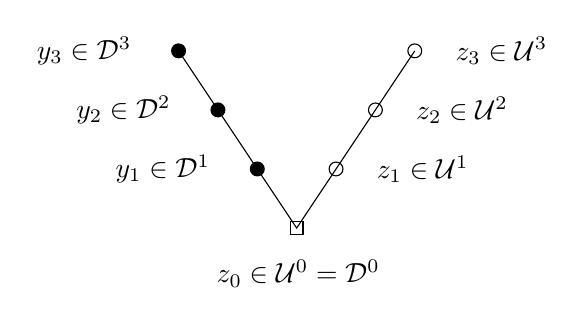
\begin{tikzpicture}[scale=1.0]
  \pgfmathsetmacro\hstep{0.5}
  \pgfmathsetmacro\vstep{0.75}
  \pgfmathsetmacro\ceps{0.08}   % size of square for coarse grid

% V-cycle with MCD down-obstacle and up-obstacle annotations
  \draw[black,thin] (-\hstep,3*\vstep) -- (0.0,2*\vstep) -- (\hstep,\vstep) --  (2*\hstep,0.0)
                    -- (3*\hstep,\vstep) -- (4*\hstep,2*\vstep) -- (5*\hstep,3*\vstep);
  \filldraw (-\hstep,3*\vstep) node[xshift=-12mm] {$y_3 \in \mathcal{D}^3$} circle (2.5pt);
  \filldraw (0.0,2*\vstep) node[xshift=-12mm] {$y_2 \in \mathcal{D}^2$} circle (2.5pt);
  \filldraw (\hstep,\vstep) node[xshift=-12mm] {$y_1 \in \mathcal{D}^1$} circle (2.5pt);
  \draw     (2*\hstep-\ceps,-\ceps) node[xshift=1mm,yshift=-5mm] {$z_0 \in \mathcal{U}^0 = \mathcal{D}^0$} rectangle (2*\hstep+\ceps,+\ceps);
  \draw     (3*\hstep,\vstep) node[xshift=11mm] {$z_1 \in \mathcal{U}^1$} circle (2.5pt);
  \draw     (4*\hstep,2*\vstep) node[xshift=11mm] {$z_2 \in \mathcal{U}^2$} circle (2.5pt);
  \draw     (5*\hstep,3*\vstep) node[xshift=11mm] {$z_3 \in \mathcal{U}^3$} circle (2.5pt);
\end{tikzpicture}

\end{center}
\caption{The FASCD V-cycle computes downward corrections $y_j \in \mathcal{D}^j$, but the upward corrections $z_j\in\mathcal{U}^j$ are in larger sets.}
\label{fig:fascdvcycle}
\end{figure}

A key idea is that, because $\mathcal{U}^j\supset \mathcal{D}^j$, up-smoothing solves less-restricted VI problems than down-smoothing.  Intuitively-speaking, going downward one does not know what the next coarse corrections will be, thus they must be in small sets $\mathcal{D}^j$, so that their sum is admissible once we return to a given level.  On the other hand, going upward no further coarse corrections can violate admissibility.

To state the V-cycle algorithm below we must also clarify the problems solved at each mesh level.  As in FAS multigrid for nonlinear PDEs \cite{BrandtLivne2011,Bruneetal2015,Trottenbergetal2001}, both the solution approximation and the residual must be coarsened, and a source functional created.  On mesh level $j$ we assume a re-discretized nonlinear operator $f^j$, with output in $(\cV^j)'$, which is an FE discretization of $f$ in \eqref{eq:boxdirichletvi}, presumably using quadrature etc.~by the same scheme which generated $f^J$ in \eqref{eq:fe:vi}.  Note that finest-level problem \eqref{eq:fe:vi} uses the original source functional $\ell^J$.  An admissible iterate $w^J \in \mathcal{K}^J$ has already\footnote{In practice the LDCs $\underline{\chi}^j,\overline{\chi}^j,\underline{\phi}^j,\overline{\phi}^j$ are generated during the descent stage; see Algorithm \ref{alg:fascd}.} been used to generate the LDCs and constraint sets $\mathcal{D}^j$, $\mathcal{U}^j$ at each level (Section \ref{sec:cdmultilevel}); these LDCs do not depend on the coarse-level corrections.

As we descend we define new $j$th-level iterates
\begin{equation}
w^j = \iR(w^{j+1} + y^{j+1}).  \label{eq:fe:definew}
\end{equation}
(These are the states \emph{before} smoothing and/or correction.)  From $w^j$ we define $\ell^j \in (\cV^j)'$:
\begin{equation}
\ell^j = \begin{cases} \ell^J, & j=J \\
                       f^j(w^j) + R\left(\ell^{j+1}-f^{j+1}(w^{j+1}+y^{j+1})\right), & j<J. \end{cases} \label{eq:fe:levelsource}
\end{equation}
Observe that injection $\iR$ coarsens the iterates---injection is commonly used in classical FAS \cite[section 5.3]{Trottenbergetal2001}---but canonical restriction $R$ coarsens linear functionals.\footnote{Recall that Table \ref{tab:transfers} summarizes our transfer operators.}

On descent, at levels $j=J,J-1,\dots,1$, we solve the following VI for $y^j \in \mathcal{D}^j$:
\begin{equation}
\ip{f^j(w^j + y^j)}{v-y^j} \ge \ip{\ell^j}{v-y^j} \qquad \text{for all } v\in \mathcal{D}^j, \label{eq:fe:downvi}
\end{equation}
for which the initial iterate is $y_{(0)}^j=0$.  (Zero is admissible; see the comment after \eqref{eq:fe:philevels}.)  On ascent, $j=0,1,\dots,J$, the same VI is solved but for $z^j \in \mathcal{U}^j$, in a larger admissible set:
\begin{equation}
\ip{f^j(w^j + z^j)}{v-z^j} \ge \ip{\ell^j}{v-z^j} \qquad \text{for all } v\in \mathcal{U}^j. \label{eq:fe:upvi}
\end{equation}
The nontrivial initial iterate for this problem is found by prolonging $z^{j-1}$ and using it to correct the current (i.e.~down-smoothed) correction on the level:\footnote{Prolongation $P$ in \eqref{eq:fe:upwardinitial} reflects the change in FE representation.}
\begin{equation}
z_{(0)}^j = y^j + P z^{j-1}.  \label{eq:fe:upwardinitial}
\end{equation}
An exception is that $z_{(0)}^0=0$ on the coarsest level.  Note $z_{(0)}^j$ is admissible since $\mathcal{D}^j + \mathcal{U}^{j-1} \subset \mathcal{U}^j$; see \eqref{eq:fe:upwardsuminclusion}.

If we were to inject the original box constraints \eqref{eq:fe:fineconstraintset} downward to coarser meshes, i.e.~$\underline{\gamma}^j = \iR \underline{\gamma}^{j+1}$ and $\overline{\gamma}^j = \iR \overline{\gamma}^{j+1}$, then, because injection preserves inequalities, and because $y^{j+1} \in \mathcal{D}^{j+1}$, it would follow from \eqref{eq:fe:definew} that $\underline{\gamma}^j \le w^j \le \overline{\gamma}^j$.  In this sense $w^j$ is admissible with respect to the box constraints.  However, while $w^j \in \cV^j \subset \cV^J$ holds, generally $w^j \notin \cK^J$, and furthermore, following \cite{GraeserKornhuber2009}, our use of LDCs (Table \ref{tab:ldcs}) avoids the need to generate these $\underline{\gamma}^j, \overline{\gamma}^j$.  In any case, Algorithm \ref{alg:fascd} yields a new finest-level iterate $w^J+z^J \in \cK^J$ which is  admissible for problem \eqref{eq:fe:vi}.

Observe that formula \eqref{eq:fe:levelsource} for functional $\ell^j$ is a classical FAS construction; compare equation (8.5b) in \cite{BrandtLivne2011} or equation (5.3.14) in \cite{Trottenbergetal2001}.  It has the following explanation, mimicking the PDE version, which simultaneously justifies VI problems \eqref{eq:fe:downvi} and \eqref{eq:fe:upvi}.  First, the $j+1$ level problem \eqref{eq:fe:downvi} is not solved exactly by the finer-level correction $y^{j+1}$---the down-smoother was only approximate---so we seek a further correction $y$ on the $j+1$ level such that
\begin{equation}
\ip{f^{j+1}(w^{j+1}+y^{j+1}+y)}{v-y^{j+1}-y} \ge \ip{\ell^{j+1}}{v-y^{j+1}-y} \quad \text{\emph{(notional)}} \label{eq:fe:downvinotional}
\end{equation}
for all $v\in \mathcal{D}^j$.  However, in fact $y$ will be approximated by solving a coarser, $j$th-level problem generated by modifying \eqref{eq:fe:downvinotional} in 4 steps:
\begin{enumerate}
\item subtract the computable quantity $f^{j+1}(w^{j+1}+y^{j+1}) \in (\mathcal{V}^{j+1})'$ from both sides,
\item replace the residual $\ell^{j+1}-f^{j+1}(w^{j+1}+y^{j+1})$ on the right by its restriction,
\item replace $w^{j+1}+y^{j+1}$, where it appears on the left, by its restriction, and
\item where it appears on the left, replace $f^{j+1}$ by the coarser rediscretization $f^j$.
\end{enumerate}
Steps \emph{(ii)}--\emph{(iv)} are justified when the residual and the error are smooth; such smoothness should result from application of the down-smoother.  These steps yield a problem for the $j$th-level correction $y^j \in \mathcal{D}^j$:
\begin{align}
&\ip{f^j\left(\iR(w^{j+1}+y^{j+1})+y^j\right)}{v-y^j} - \ip{f^j\left(\iR(w^{j+1}+y^{j+1})\right)}{v-y^j} \label{eq:fe:downvicluttered} \\
&\qquad \ge \ip{R\left(\ell^{j+1}-f^{j+1}(w^{j+1}+y^{j+1})\right)}{v-y^j} \notag
\end{align}
This is the same as VI problem \eqref{eq:fe:downvi}, but in cluttered form; definitions \eqref{eq:fe:definew} and \eqref{eq:fe:levelsource} create \eqref{eq:fe:downvi}.  The explanation for VI \eqref{eq:fe:upvi} is similar.

We will regard the smoothers for VI problems \eqref{eq:fe:downvi} and \eqref{eq:fe:upvi} as approximate, in-place procedures, acting on the corrections $y^j$ and $z^j$, respectively (Section \ref{sec:implementation}).  Also, as is standard in multigrid, at the coarsest $j=0$ level we suppose that problem \eqref{eq:fe:upvi} is solved accurately.

These ideas come together in Algorithm \ref{alg:fascd}, \pr{fascd-vcycle}, which acts in-place on $w^J$.  It assumes certain semantics for the \pr{smooth} and the coarsest-level \pr{solve} procedures; they do in-place modifications of their final arguments, without modifying their first four arguments.  Parameters \id{down} and \id{up} determine the number of smoother iterations, respectively.

\begin{pseudofloat}[ht]
\begin{pseudo}
\pr{fascd-vcycle}(\ell^J,\underline{\gamma}^J,\overline{\gamma}^J;w^J)\text{:} \\+
    $\underline{\chi}^J = \underline{\gamma}^J - w^J {\large \strut}$ \\
    $\overline{\chi}^J = \overline{\gamma}^J - w^J {\large \strut}$ \\
    for $j=J$ downto $j=1$ \\+
      $\underline{\chi}^{j-1} = \maxR \underline{\chi}^j {\large \strut}$ \\
      $\overline{\chi}^{j-1} = \minR \overline{\chi}^j {\large \strut}$ \\
      $\underline{\phi}^j = \underline{\chi}^j - P\underline{\chi}^{j-1} {\large \strut}$ \\
      $\overline{\phi}^j = \overline{\chi}^j - P\overline{\chi}^{j-1} {\large \strut}$ \\
      $y^j = 0$ \\
      $\text{\pr{smooth}}^{\text{\id{down}}}(\ell^j,\underline{\phi}^j,\overline{\phi}^j,w^j;y^j)$  \ct{smoothing of \eqref{eq:fe:downvi} in $\mathcal{D}^j$}\\
      $w^{j-1} = \iR(w^j + y^j)$ \\
      $\ell^{j-1} = f^{j-1}(w^{j-1}) + R \left(\ell^j - f^j(w^j+y^j)\right)$ \\-
    $z^0 = 0$ \\
    $\text{\pr{solve}}(\ell^0,\underline{\chi}^0,\overline{\chi}^0,w^0;z^0)$ \hspace{1.0cm} \ct{solving of \eqref{eq:fe:upvi} in $\mathcal{U}^0$} \\
    for $j=1$ to $j=J$ \\+
      $z^j = y^{j} + P z^{j-1}$ \\
      $\text{\pr{smooth}}^{\text{\id{up}}}(\ell^j,\underline{\chi}^j,\overline{\chi}^j,w^j;z^j)$  \ct{smoothing of \eqref{eq:fe:upvi} in $\mathcal{U}^j$} \\-
    $w^J \gets w^J+z^J$
\end{pseudo}
\caption{The FASCD V-cycle is an iteration for solving FE VI problem \eqref{eq:fe:vi}.  Here $f^j$ denotes an FE discretization of $f$ in problem \eqref{eq:boxdirichletvi}.}
\label{alg:fascd}
\end{pseudofloat}

Compared specifically to the $V(1,0)$ cycle presented as Algorithm 4.7 in \cite{GraeserKornhuber2009}, one might say informally that \pr{fascd-vcycle} is a $V(1,1)$ cycle.  However, its structure relates directly to the basic CD iterations (Sections \ref{sec:cd}) as well.  In unilateral cases it is precise to say that one iteration of \pr{fascd-vcycle} is an application of \pr{cd-mult} over CD \eqref{eq:fe:downwardsuminclusion}, using the defect constraint meaning of the downward constraint sets $\mathcal{D}^j$, followed by an application of \pr{icd-tele} (Section \ref{sec:cdmultilevel}) over the incomplete CD \eqref{eq:fe:upwardsuminclusion}.  FIXME: idea is that once you are using defect constraints you no longer depend on the literal availability of $\Pi_i$, so incomplete CD suffices, e.g.~even for \pr{cd-mult}

Regarding storage required for \pr{fascd-vcycle}, and assuming all box constraints are nontrivial, 7 vectors must be allocated on each level: $\underline{\chi}^j$, $\overline{\chi}^j$, $\underline{\phi}^j$, $\overline{\phi}^j$, $w^j$, $\ell^j$, $y^j$.  Note $z^j$ can use the same storage as $y^j$.  On the finest level one must also store $\underline{\gamma}^J$ and $\overline{\gamma}^J$, while on the coarsest level there are only 5 vectors because $\underline{\phi}^0=\underline{\chi}^0$ and $\overline{\phi}^0=\overline{\chi}^0$.  Therefore, using $m_j=2^d m_{j-1}$, plus a geometric series argument, the total floating-point storage, excluding smoother and coarse-solver implementations, is
\begin{equation}
9 m_J + 7 m_{J-1} + \dots + 7 m_1 + 5 m_0 \le \left(9 + \frac{7}{2^d - 1}\right) m_J.
\end{equation}
This gives storage at most $16m_J$, $12m_J$, and $10m_J$ in dimensions $d=1,2,3$, respectively.  For comparison, a single-level method needs $4 m_J$ storage.\footnote{That is, for vectors $\underline{\gamma}^J,\overline{\gamma}^J,\ell^J,w^J$.}  If some of the obstacles are trivial, for instance in the unilateral case $\overline{\gamma}^J=+\infty$, storage is reduced at all levels.


\section{Implementation and smoothers} \label{sec:implementation}

In this section we consider several practical concerns when implementing and applying \pr{fascd-vcycle} Algorithm \ref{alg:fascd}.  We address convergence criteria, smoothers, and coarse solvers, plus the F-cycle extension of the Algorithm, sometimes called a \emph{full multigrid cycle}.

Because the problem is inequality-constrained, repeated application of \pr{fascd-vcycle} to solve the finite-dimensional, box-constrained VI \eqref{eq:fe:vi} will not generally reduce the residual $f^J(w^J) - \ell^J$ to zero everywhere.  However, \eqref{eq:fe:vi} is equivalent to a \emph{mixed complementarity problem} (MCP) \cite{FacchineiPang2003}, a strong form amenable to convergence criteria.  Let $x_p \in \mathcal{T}^J$ be a finest-level node, and $\psi_p(x)$ the corresponding hat function.  Let $\mathcal{X}^J=\big\{w\in\cV^J\,:\,w(x_p)=g_D^J(x_p) \text{ if } x_p\in \partial_D\Omega\big\}$, thus $\cK^J = \left\{\underline{\gamma}^J \le w \le \overline{\gamma}^J\right\} \cap \mathcal{X}^J$.  If $m_D$ is the number of nodes $x_p$ in the Dirichlet boundary, let $I_D$ be the $m_D\times m_J$ matrix which extracts Dirichlet nodal values; its transpose $I_D^\top$ injects Dirichlet boundary degrees of freedom into $(\mathcal{V}^J)'$.  Finally, we will write $a\perp b$ when $a,b \in \RR^n$ are \emph{complementary}, that is, when $a_i \ge 0$ and $b_i \ge 0$ and $a_i b_i = 0$ for $i=0,\dots,n-1$.  Then problem \eqref{eq:fe:vi}, which would be expressed VI$\left(f^J(\cdot)-\ell^J,\left[\,\underline{\gamma}^J,\overline{\gamma}^J\right] \cap \mathcal{X}^J\right)$ in the operations research literature \cite{FerrisPang1997}, is equivalent to the following MCP for the solution $u^J \in \mathcal{K}^J$, but with additional equality constraints:
\begin{align}
\underline{\gamma}^J \le u^J \le \overline{\gamma}^J \quad &\perp \quad f^J(u^J) - \ell^J - I_D^\top \lambda \label{eq:fe:mcp} \\
I_D u^J &= g_D^J\big|_{\partial_D\Omega} \notag
\end{align}
for some Lagrange multipliers $\lambda \in \RR^{m_D}$.  By definition, MCP \eqref{eq:fe:mcp} says that certain node-wise conditions hold for $u^J$ at $x_p \in \mathcal{T}^J$.  If $x_p \notin \partial_D\Omega$ then one of these four conditions hold:
\begin{itemize}
\item $\underline{\gamma}^J(x_p)<u^J(x_p)<\overline{\gamma}^J(x_p)$ and $\ip{f^J(u^J)-\ell^J}{\psi_p} = 0$,
\item $\underline{\gamma}^J(x_p)=u^J(x_p)<\overline{\gamma}^J(x_p)$ and $\ip{f^J(u^J)-\ell^J}{\psi_p} \ge 0$,
\item $\underline{\gamma}^J(x_p)<u^J(x_p)=\overline{\gamma}^J(x_p)$ and $\ip{f^J(u^J)-\ell^J}{\psi_p} \le 0$,
\item $\underline{\gamma}^J(x_p)=u^J(x_p)=\overline{\gamma}^J(x_p)$.
\end{itemize}
Otherwise, if $x_p \in \partial_D\Omega$ then
\begin{itemize}
\item $u^J(x_p)=g_D^J(x_p)$ and $\lambda_p=\ip{f^J(u^J)-\ell^J}{\psi_p}$.
\end{itemize}
The cases might be labeled \emph{inactive}, \emph{lower active}, \emph{upper active}, \emph{pinched} (\emph{both active}), and \emph{boundary}, respectively.  Where \emph{pinched} applies, $\ip{f^J(u^J)-\ell^J}{\psi_p}$ can have any real value.

Thus the MCP \eqref{eq:fe:mcp} identifies expressions whose norms should go below tolerance.  For for $w^J \in \mathcal{K}^J$, let $r_p = \ip{f^J(w^J)-\ell^J}{\psi_p}$, the pointwise (ordinary) residual, as a notational convenience.  First, interpreting the MCP directly, we define the finest-level \emph{nodal complementarity residual} $\rNC$ in $\RR^{m_J}$ from the five cases:
\begin{equation}
\rNC(w^J)_p = \begin{cases}
    r_p, & \underline{\gamma}^J(x_p) < w^J(x_p) < \overline{\gamma}^J(x_p), \\
    \min\{r_p,0\}, & w^J(x_p) = \underline{\gamma}^J(x_p), \\
    \max\{r_p,0\}, & w^J(x_p) = \overline{\gamma}^J(x_p), \\
    0, & \underline{\gamma}^J(x_p)=w^J(x_p)=\overline{\gamma}^J(x_p), \\
    w^J(x_p) - g_D^J(x_p), & x_p \in \partial_D\Omega. \end{cases} \label{eq:rNC}
\end{equation}
(The first four cases assume $x_p \notin \partial_D\Omega$.)  Note that $\rNC : \mathcal{K}^J \to \RR^{m_J}$ is a computable nonlinear map defined from $f^J$ and the vectors $\ell^J$, $\underline{\gamma}^J$, and $\overline{\gamma}^J$, and that for PDEs without constraints one uses only the first and last cases.  In summary, $\rNC(w^J)_p$ is nonzero at nodes where MCP \eqref{eq:fe:mcp} is violated, either because the pointwise residual $\ip{f^J(w^J)-\ell^J}{\psi_p}$ remains nonzero where the constraints are inactive, or because it has the wrong sign at an actively-constrained degree of freedom, or because the boundary condition is not satisfied.

As a practical matter, however, direct implementation of \eqref{eq:rNC} is sensitive to rounding error because $\rNC$ is a discontinuous function of $w^J(x_p)$.  For example, if $w^J(x_p)$ exceeds $\underline{\gamma}^J(x_p)$ by $10^{-16}$, then, instead of returning the minimum of $z_p = \left<f^J(w^J)-\ell^J,\psi_p\right>$ and zero (the second case), the first case applies and $\rNC(w^J)_p = z_p$, which might be large (positive), and this would suggest falsely that the iteration is far from converging.  On the other hand, an advantage of formula \eqref{eq:rNC} is that it applies as stated if $\underline{\gamma}^J(x_p)=-\infty$ or $\overline{\gamma}^J(x_p)=+\infty$; compare \eqref{eq:rSS} below, wherein the difference $w^J(x_p) - \underline{\gamma}^J(x_p)$ is computed, for example.

%\newcommand{\phiFB}{\phi_{\text{FB}}}
We will instead measure convergence using a \emph{semi-smooth residual} based on the Fischer-Burmeister function \cite{BensonMunson2006,Ulbrich2011}, a function defined as follows for $a,b\in\RR$:
\begin{equation}
\phi(a,b) = a + b - \sqrt{a^2 + b^2}. \label{eq:phiFB}
\end{equation}
Observe that $\phi(a,b)=0$ if and only if $a,b$ are complementary, and also that $\phi$ semi-smooth (and thus continuous).  For convenience denote $\underline{g}_p = w^J(x_p) - \underline{\gamma}^J(x_p)$ and $\overline{g}_p = \overline{\gamma}^J(x_p) - w^J(x_p)$, the positive gaps at $x_p$.  Finally define
\begin{equation}
\rSS(w^J)_p = \begin{cases}
r_p, & \underline{\gamma}^J(x_p) = -\infty \text{ and } \overline{\gamma}^J(x_p) = +\infty, \\
\phi\big(\underline{g}_p, r_p\big), & \overline{\gamma}^J(x_p) = +\infty, \\
\phi\left(\overline{g}_p, -r_p\right), & \underline{\gamma}^J(x_p) = -\infty, \\
\max\big\{\phi\big(\underline{g}_p, r_p\big), \phi\left(\overline{g}_p, -r_p\right)\big\}, & \text{otherwise}, \\
w^J(x_p) - g_D^J(x_p), & x_p \in \partial_D\Omega,
\end{cases} \label{eq:rSS}
\end{equation}
where again $x_p \notin \partial_D\Omega$ in the first four cases.

Now suppose we repeatedly apply \pr{fascd-vcycle}, starting with $w^{J,0} \in \mathcal{K}^J$, generating (fine-level) iterates $w^{J,k} \in \mathcal{K}^J$.  Let $\id{atol}\ge 0$, $\id{rtol}\ge 0$ be given tolerances.  Then the criterion used in the results (Section \ref{sec:results}) is 
\begin{equation}
\|\rSS(w^{J,k})\|_2 < \id{atol} \qquad \text{or} \qquad \frac{\|\rSS(w^{J,k})\|_2}{\|\rSS(w^{J,0})\|_2} < \id{rtol} \label{eq:stoppingcriterion}
\end{equation}
A step tolerance, based on $\|w^{J,k} - w^{J,k-1}\|_2$, could also be used, but we did not find it necessary.

FIXME smoother semantics; shift ``$w^j+y^j$'' etc.

FIXME smoothers use Newton reduced space (RS) \cite{BensonMunson2006}with either direct linear solve or a fixed number of Krylov steps; in latter case either fixed number of CG+ICC for symmetric linear operator (Laplacian), otherwise fixed number of GMRES+ILU

% FIXME try Newton semi-smooth \cite{BensonMunson2006}?

FIXME F-cycles

\begin{pseudofloat}[ht]
\begin{pseudo}
\pr{fascd-fcycle} \\
FIXME
\end{pseudo}
\caption{The FASCD F-cycle for solving FE VI problem \eqref{eq:fe:vi}.}
\label{alg:fascd-fcycle}
\end{pseudofloat}


\section{Results} \label{sec:results}

Algorithms \ref{alg:fascd} and \ref{alg:fascd-fcycle} were implemented in Python using the Firedrake library \cite{Rathgeberetal2016}.  In this Section we show numerical results for the several VI Examples in Section \ref{sec:vi}, with a focus on the scaling of FASCD iterations as the mesh resolution increases.  Assuming strong, yet $O(m_J)$ arithmetic, smoothers on each level, as illustrated below, our essential observations are that each V-cycle dramatically reduces the residual norm, and that a couple of F-cycles solves most Examples down to discretization error.

\begin{example} \label{ex:results:classical}
Consider the 2D classical, i.e.~unilateral and Laplacian, obstacle problem, namely Example \ref{ex:plaplacian} with $p=2$ and admissible set $\mathcal{K} = \{v \ge \psi\} \subset W^{1,2}(\Omega)$.  We consider two problems with very different coincidence (active) sets $\{x\in\Omega \,:\, u(x)=\psi(x)\}$, both over square $\Omega$.   The standard ``ball'' problem has an upper hemisphere obstacle $\psi$ \cite[Chapter 12]{Bueler2021}.  In the ``spiral'' problem from Example 7.1.1 in \cite{GraeserKornhuber2009}, $\psi$ is constructed to produce a more interesting coincidence set; see Figure \ref{fig:results:classical}.  Note that $\psi\big|_{\partial \Omega} \le 0$ in both problems.

For this experiment we used $P_1$ elements, standard uniform mesh refinement, and a coarsest mesh of $m_0=5^2$ nodes (32 triangles).  The finest mesh had $m_9=2049^2 \approx 4.2 \times 10^{6}$ nodes.  As our smoother we applied a single RS Newton iteration (Section \ref{sec:implementation}), with three (fixed) ICC-preconditioned CG iterations to approximately solve the step equations.  The coarse solver was RS$+$LU, iterated to convergence.  Tolerances \texttt{rtol} $= 10^{-6}$ and \texttt{atol} $= 10^{-12}$ were used in stopping criterion \eqref{eq:stoppingcriterion}.  The initial iterate was set to $w=\max\{0,\psi\}$.

Table \ref{tab:results:classical} shows the resulting iteration counts.  When the RS Newton smoother is applied by itself as a solver it shows rapidly-increasing iterations as expected, roughly proportional to resolution.  By contrast, V-cycle iterations increase slowly, perhaps logarithmically with the resolution.  Noting that for F-cycles we are counting the number of V-cycles after the ramp (Section \ref{sec:implementation}), we see that a constant number of cycles solves the problem.  The spiral problem appears to be only slightly more challenging for these solvers.  The complexity of the coincidence set or free boundary does not strongly-influence FASCD performance.

Each V-cycle does the work of about eight finest-level preconditioned Krylov (CG+ICC) iterations.  For the F-cycle results, where three iterations suffice at all resolutions in either problem, this is close to textbook multigrid efficiency\footnote{Textbook multigrid efficiency is imperfectly defined, but consider \cite{BrownSmithAhmadia2013}: ``an order of magnitude reduction in residual per iteration and solution of the fine-level system at a small multiple of the cost of a residual evaluation.''  However, work of at most ten residual evaluations is often mentioned.} despite the low solution regularity.
\end{example}

%REGENERATE using git@bitbucket.org:pefarrell/fascd.git, in examples/
%$ timer python3 drape.py -prob ball|spiral -levs 9 -o ball|spiral.pvd -fascd_rtol 1.0e-6 -fascd_atol 1.0e-6 -fascd_cycle_type full
%$ paraview ball|spiral.pvd
%use preset "xray" and invert colors
\begin{figure}[ht]
\begin{center}
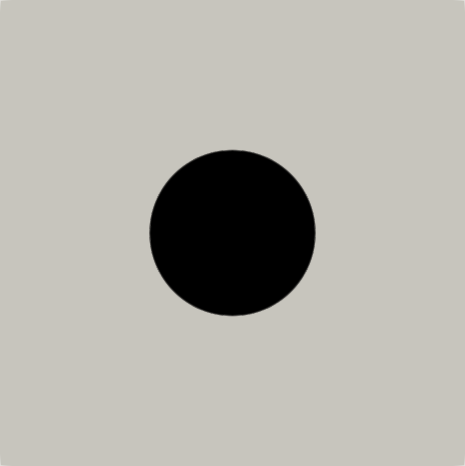
\includegraphics[width=0.35\textwidth]{fixfigs/ball-set.png} \qquad 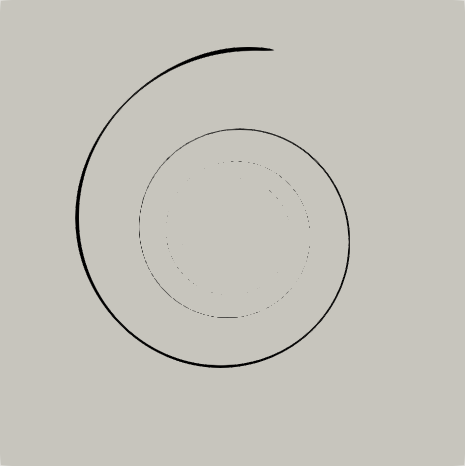
\includegraphics[width=0.35\textwidth]{fixfigs/spiral-set.png}
\end{center}
\caption{Coincidence sets (black) for the ball and spiral problems in Example \ref{ex:results:classical}.}
\label{fig:results:classical}
\end{figure}

% see git@bitbucket.org:pefarrell/fascd.git: examples/drape.py and edplay/results/drape.sh|txt
\begin{table}[ht]
\begin{tabular}{lr@{\hskip 7mm}cccccc}
\multirow{2}{*}{\emph{levels}} & \multirow{2}{*}{$m_J$} & \multicolumn{3}{c}{\,\emph{ball}} & \multicolumn{3}{c}{\,\emph{spiral}} \\ \cmidrule(lr){3-5} \cmidrule(lr){6-8}
   &          & V-cycle & F-cycle & RS only & V-cycle & F-cycle & RS only \\ \cmidrule{1-8}
 1 &    $5^2$ &  1 &  1 &  1  &  1 &  1 &  1 \\
 2 &    $9^2$ &  2 &  1 &  2  &  2 &  1 &  2 \\
 3 &   $17^2$ &  2 &  2 &  3  &  3 &  2 &  4 \\
 4 &   $33^2$ &  3 &  2 &  6  &  3 &  2 &  7 \\
 5 &   $65^2$ &  3 &  2 &  8  &  4 &  3 &  9 \\
 6 &  $129^2$ &  4 &  2 & 17  &  4 &  3 & 16 \\
 7 &  $257^2$ &  4 &  2 & 33  &  4 &  3 & 27 \\
 8 &  $513^2$ &  5 &  2 & 65  &  5 &  3 & 48 \\
 9 & $1025^2$ &  5 &  2 & \XX &  5 &  3 & \XX \\
10 & $2049^2$ &  5 &  2 & \XX &  5 &  3 & \XX
\end{tabular}
\bigskip
\caption{Iterations for FASCD V-cycle and F-cycle algorithms in Example \ref{ex:results:classical}.  Smoother-only runs marked \XX\xspace were not attempted.}
\label{tab:results:classical}
\end{table}

\begin{example}  \label{ex:results:plap}
Recall Example \ref{ex:plaplacian}, the nonlinear $p$-Laplacian operator.  Here we consider a unilateral obstacle problem, in one dimension for visualizability, for both fast ($p=1.5$) and degenerate ($p=4.0$) diffusivity cases.\footnote{``Fast'' and ``degenerate'' refer to $D=|\grad u|^{p-2}\to \infty$ and $D\to 0$ as $|\grad u|\to 0$, respectively.  Ellipticity is lost in the latter case.  For such $p$-Laplacian obstacle problems, well-posedness and ($p$-dependent) solution regularity are considered in \cite{ChoeLewis1991}.}  This example reveals the sometimes strong contrast between $V(1,0)$ and $V(0,1)$ results, namely \pr{up} $=0$ and \pr{down} $=0$ in Algorithm \ref{alg:fascd}, and it emphasizes the need for robust smoothers.

Suppose $\Omega=(-3,3)$, $\psi(x) = -0.2|x|$, $\mathcal{K} = \{v \ge \psi\} \subset W^{1,p}(\Omega)$, and $\ell(v) = \int_\Omega g v$ where $g(x)=1$ for $|x|<1$ and $g(x)=-1$ for $|x|>1$.  The exact solution of VI \eqref{eq:vi} is easily computed for any $p$; see Figure \ref{fig:results:plap}.  For this experiment we used $P_1$ elements, a coarsest mesh of $m_0=7$ nodes, and nine standard refinements to a $m_9=3073$ finest mesh.  The default smoother uses three (fixed) iterations of RS Newton, with LU solution of the step equations.\footnote{This is an optimal $O(m_j)$ smoother in 1D.}  The coarse solver is the same but iterated to convergence.  The initial iterate was $w=\psi$, and again \texttt{rtol} $= 10^{-6}$ and \texttt{atol} $= 10^{-12}$.

%REGENERATE using elbueler/plapfigs branch of git@bitbucket.org:pefarrell/fascd.git, in examples/
% $ python3 plap1d.py -p 1.5 -figures -levs 6 -fascd_cycle_type full && mv solution.pdf plap1d1p5.pdf
% $ python3 plap1d.py -p 4.0 -figures -levs 6 -fascd_cycle_type full && mv solution.pdf plap1d4p0.pdf
\begin{figure}[ht]
\begin{center}
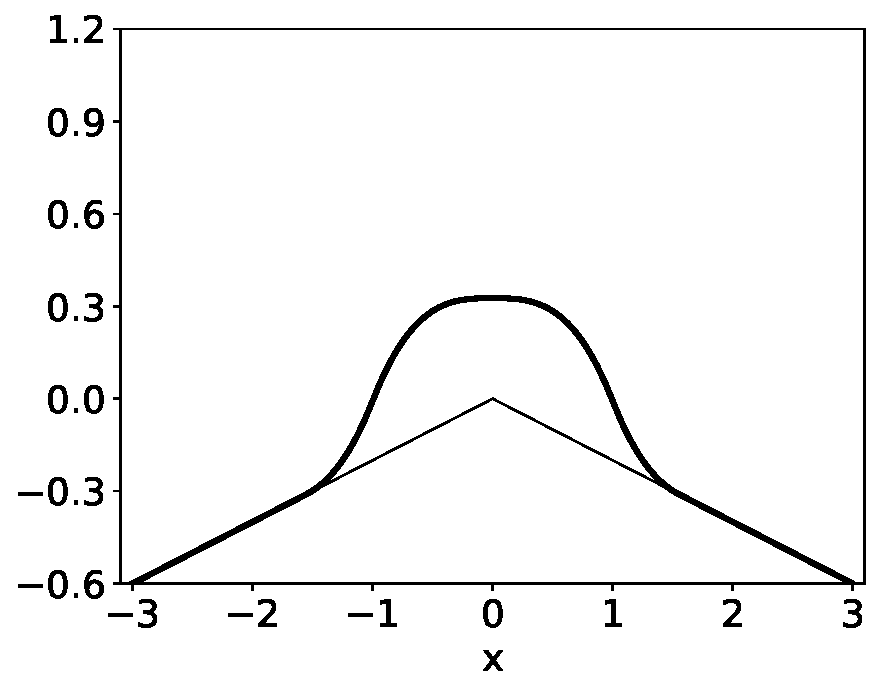
\includegraphics[width=0.45\textwidth]{fixfigs/plap1d1p5.pdf} \quad
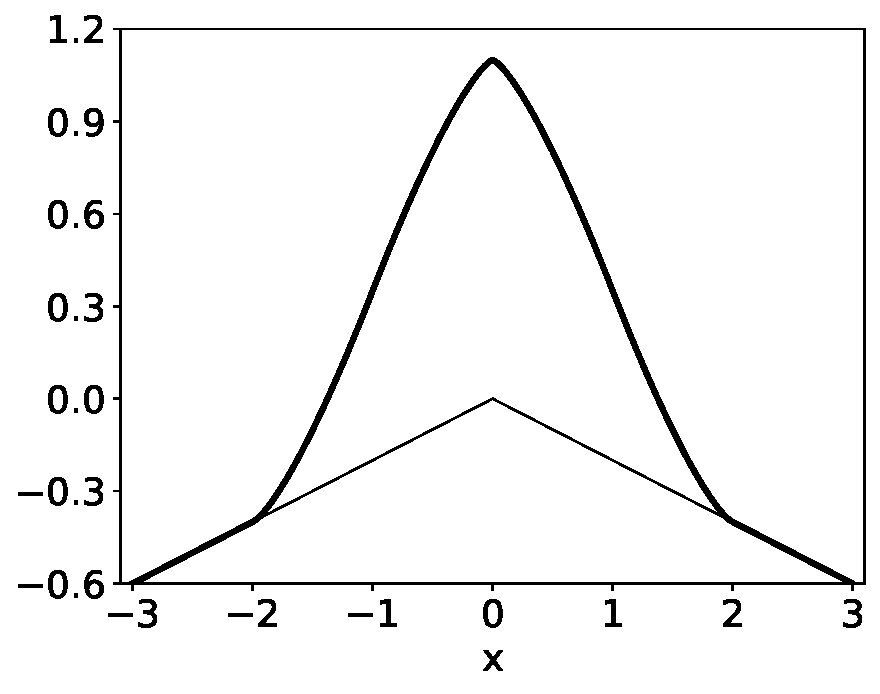
\includegraphics[width=0.45\textwidth]{fixfigs/plap1d4p0.pdf}
\end{center}
\caption{Solutions $u\ge \psi$ of the $p$-Laplacian VI in Example \ref{ex:results:plap}, for $p=1.5$ (left) and $p=4.0$ (right).}
\label{fig:results:plap}
\end{figure}

Figure \ref{fig:imagesvcycle} illustrates the major steps of an example V-cycle, showing each of the nonlinear FAS coarse correction VI subproblem solutions.  That is, each $y^j \in \mathcal{D}^j$ and $z^j \in \mathcal{U}^j$ is drawn, along with each level defect constraint $\underline{\phi}^j,\underline{\chi}^j$.

% figures in the following visualization were generated using branch elbueler/simplefigs
% of git@bitbucket.org:pefarrell/fascd.git, and the following commands:
%   cd examples/
%   python3 plap1d.py -figures -fascd_max_it 2 -fascd_cycle_type multiplicative -mcoarse 2
\begin{figure}[ht]
\begin{center}
\begin{tikzpicture}[scale=1.0]
    \pgfmathsetmacro{\HEIGHT}{2}
    \pgfmathsetmacro{\XSTEP}{3.7}
    \pgfmathsetmacro{\YSTEP}{3.7}
    \pgfmathsetmacro{\YLABEL}{-0.4}
    \pgfmathsetmacro{\NUDGE}{0.5}
    \node (start2) [] at (0,2*\YSTEP) {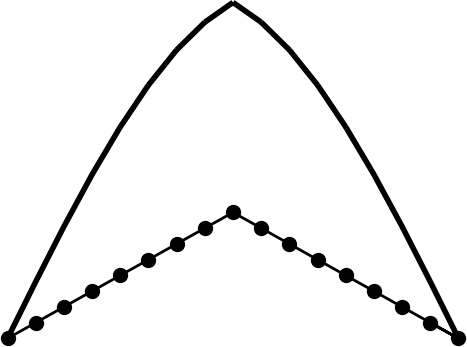
\includegraphics[height=\HEIGHT cm]{fixfigs/vcycle/start2.png}};
    \node (start2label) [below of = start2, yshift=\YLABEL cm] {$w^2 \ge \underline{\gamma}^2$};
    \node (down2) [] at (1.0*\XSTEP,2*\YSTEP) {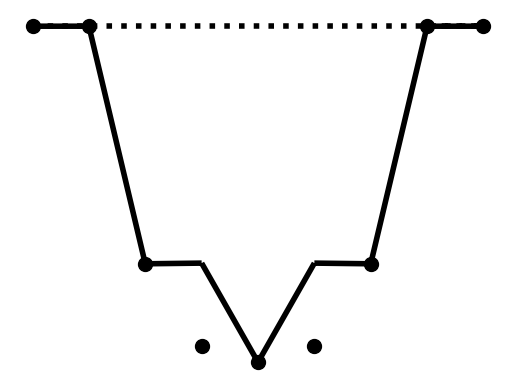
\includegraphics[height=\HEIGHT cm]{fixfigs/vcycle/down2.png}};
    \node (down2label) [below of = down2, yshift=\YLABEL cm] {$y^2 \ge \underline{\phi}^2$};
    \node (down1) [] at (1.4*\XSTEP,1*\YSTEP) {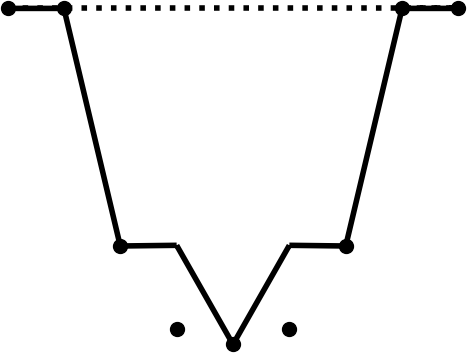
\includegraphics[height=\HEIGHT cm]{fixfigs/vcycle/down1.png}};
    \node (down1label) [below of = down1, yshift=\YLABEL cm] {$y^1 \ge \underline{\phi}^1$};
    \node (up0) [] at (1.9*\XSTEP,0) {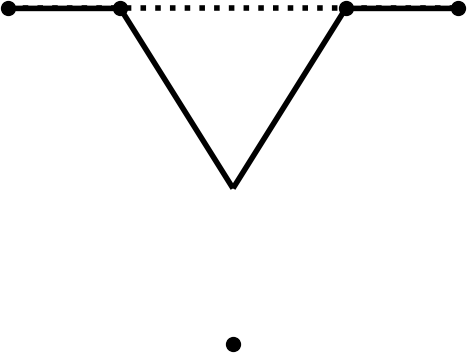
\includegraphics[height=\HEIGHT cm]{fixfigs/vcycle/up0.png}};
    \node (up0label) [below of = up0, yshift=\YLABEL cm] {$z^0 \ge \underline{\chi}^0$};
    \node (up1) [] at (2.4*\XSTEP,1*\YSTEP) {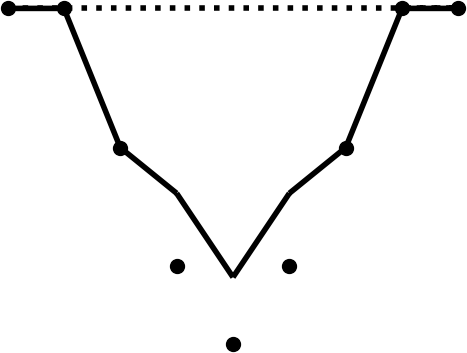
\includegraphics[height=\HEIGHT cm]{fixfigs/vcycle/up1.png}};
    \node (up1label) [below of = up1, yshift=\YLABEL cm] {$z^1 \ge \underline{\chi}^1$};
    \node (up2) [] at (2.8*\XSTEP,2*\YSTEP) {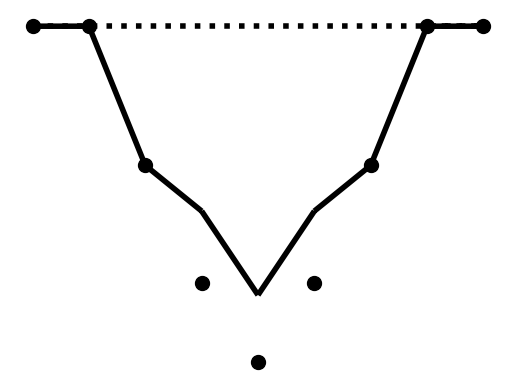
\includegraphics[height=\HEIGHT cm]{fixfigs/vcycle/up2.png}};
    \node (up2label) [below of = up2, yshift=\YLABEL cm] {$z^2 \ge \underline{\chi}^2$};
    \node (next2) [] at (3.8*\XSTEP,2*\YSTEP) {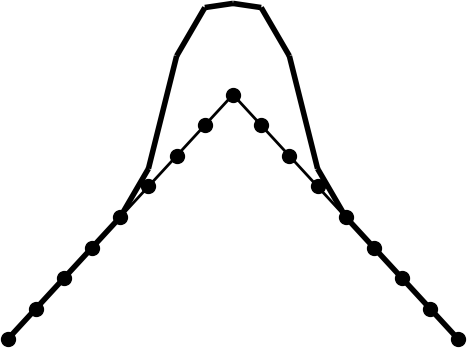
\includegraphics[height=\HEIGHT cm]{fixfigs/vcycle/next2.png}};
    \node (next2label) [below of = next2, yshift=\YLABEL cm] {$\tilde{w}^2 \ge \underline{\gamma}^2$};
    \graph [edges = {very thick}] {
        (start2) -> (down2)
                 -!- [] (down2label) -> (down1)
                 -!- [] (down1label) -> (up0)
                 -> (up1label) -!- (up1)
                 -> (up2label) -!- (up2)
                 -> (next2)
    };
\end{tikzpicture}

\end{center}
\caption{Visualization of one FASCD V-cycle iteration for Example \ref{ex:results:plap}, with $p=1.5$, $J=3$, and a coarsest mesh of $m_0=3$ nodes.  Solutions (i.e.~$w^j$, $y^j$, $z^j$) are lines while obstacles ($\underline{\gamma}^j$, $\underline{\phi}^j$, $\underline{\chi}^j$) are strong dots.  The zero function (dotted) is the admissible initial iterate for $y^j$ and $z^j$.  Vertical scale varies.}
\label{fig:imagesvcycle}
\end{figure}

Iteration results are shown in Table \ref{tab:results:fastplap1d} for the fast diffusion $p=1.5$ case.  We see that $V(1,0)$ cycles, essentially Algorithm 4.7 in \cite{GraeserKornhuber2009} but with a stronger smoother, often do not converge.  By contrast, $V(0,1)$ cycles, using only up-smoothing in the larger sets $\mathcal{U}^j$ (Section \ref{sec:cdmultilevel}), are just as good as the default $V(1,1)$ cycles (i.e.~Algorithm \ref{alg:fascd}).  F-cycles are even more efficient except when they fail entirely, but the failures arise from singular diffusivity.  If we regularize  $D=|\grad u|^{-0.5}$ to $D_\eps = \left(\eps + |\grad u|^2\right)^{-0.25}$, with $\eps=10^{-8}$, then a single F-cycle suffices at every resolution (column ``F$_\eps$'').

Iteration results for the (unregularized) degenerate diffusion $p=4.0$ case are in Table \ref{tab:results:degenerateplap1d}.  V-cycles using the default settings, specifically three fixed RS Newton iterations, do not converge on the finer meshes; the semi-smooth NCP residual norms \eqref{eq:stoppingcriterion} are unbounded in the failed runs.  Visualization shows an instability in which oscillations in the restricted residuals explode.  However, either a slight increase in smoother power, to four RS Newton iterations, or improved finest-level initial iterates through use of an F-cycle, stops the instability.  Even for the three-iteration solver, a single F-cycle suffices at every resolution.

The $p=1.5$ and $p=4$ cases give different convergence rates in the $\|\cdot\|_\infty$ norm, namely at rates $O(h^{2.005})$ and $O(h^{1.420})$, respectively.
\end{example}

% see git@bitbucket.org:pefarrell/fascd.git: examples/plap1d.py and edplay/results/plap1d.sh|txt
\begin{table}[ht]
\begin{tabular}{lr@{\hskip 7mm}c@{\hskip 3mm}c@{\hskip 3mm}c@{\hskip 4mm}c@{\hskip 5mm}c@{\hskip 6mm}c}
\emph{levels} & $m_J$ & V(1,0) & V(0,1) & V(1,1) & F & F$_\eps$ & $\|$error$\|_\infty$ \\ \cmidrule{1-8}
 1 &    $7$ &  1 &  1 &  1 &  1 &  1 & $2.3\times 10^{-1}$ \\
 2 &   $13$ &  3 &  3 &  2 &  2 &  1 & $3.3 \times 10^{-2}$ \\
 3 &   $25$ & 12 &  4 &  2 &  1 &  1 & $9.1 \times 10^{-3}$ \\
 4 &   $49$ & NC &  4 &  2 &  1 &  1 & $3.2 \times 10^{-3}$ \\
 5 &   $97$ & NC &  3 &  3 &  1 &  1 & $5.5 \times 10^{-4}$ \\
 6 &  $193$ & NC &  3 &  3 & NC &  1 & $1.7 \times 10^{-4}$ \\
 7 &  $385$ & NC &  3 &  3 &  1 &  1 & $4.7 \times 10^{-5}$ \\
 8 &  $769$ & NC &  4 &  7 &  1 &  1 & $9.5 \times 10^{-6}$ \\
 9 & $1537$ & NC &  5 &  6 & NC &  1 & $3.6 \times 10^{-6}$ \\
10 & $3073$ & NC & 11 & 19 &  1 &  1 & $4.9 \times 10^{-7}$
\end{tabular}
\bigskip
\caption{Iterations for V- and F-cycles on the $p=1.5$ problem in Example \ref{ex:results:plap}.  NC $=$ did not converge after 50 iterations.  See text regarding F$_\eps$ and error.}
\label{tab:results:fastplap1d}
\end{table}

% see git@bitbucket.org:pefarrell/fascd.git: examples/plap1d.py and edplay/results/plap1d.sh|txt
\begin{table}[ht]
\begin{tabular}{lr@{\hskip 7mm}c@{\hskip 4mm}c@{\hskip 4mm}c@{\hskip 6mm}c}
\emph{levels} & $m_J$ & V & V$_4$ & F & $\|$error$\|_\infty$ \\ \cmidrule{1-6}
 1 &    $7$ &  1 &  1 &  1 & $8.7 \times 10^{-2}$ \\
 2 &   $13$ &  1 &  1 &  1 & $3.8 \times 10^{-2}$ \\
 3 &   $25$ &  2 &  1 &  1 & $1.6 \times 10^{-2}$ \\
 4 &   $49$ &  4 &  2 &  1 & $6.3 \times 10^{-3}$ \\
 5 &   $97$ & NC &  2 &  1 & $2.3 \times 10^{-3}$ \\
 6 &  $193$ & NC &  1 &  1 & $7.0 \times 10^{-4}$ \\
 7 &  $385$ & NC &  2 &  1 & $2.0 \times 10^{-4}$ \\
 8 &  $769$ & NC &  2 &  1 & $1.1 \times 10^{-4}$ \\
 9 & $1537$ & NC &  2 &  1 & $4.0 \times 10^{-5}$ \\
10 & $3073$ & NC &  2 &  1 & $1.5 \times 10^{-5}$
\end{tabular}
\bigskip
\caption{Iterations for V- and F-cycles on the $p=4.0$ problem in Example \ref{ex:results:plap}.  See text regarding V$_4$ and error.}
\label{tab:results:degenerateplap1d}
\end{table}

Solvers implemented in Firedrake can exploit parallel solvers from the PETSc library \cite{Balayetal2023}.  In fact, the above Examples, which were run in serial so as to fix the smoother,\footnote{The action of parallel preconditioners generally depends on the number of processes \cite[for example]{Bueler2021}.} also run efficiently in parallel.  The next Example applies a parallel solver, and Example \ref{ex:results:sia} also demonstrates the parallel weak scaling \cite{Bueler2021} of FASCD.

\begin{example}  \label{ex:results:advdiff}
The advection-diffusion operator in Example \ref{ex:advectiondiffusion} is coercive when the velocity $\bX$ is divergence-free.  We now demonstrate FASCD F-cycles on such a VI problem over $\Omega=(-1,1)^d$ ($d=2,3$).  The 2D problem satisfies the coercivity hypotheses ($\bX = (7+5y,-5x)$ is divergence-free), but the 3D problem has a more general velocity ($\grad\cdot\bX \ne 0$); note $u=0$ on all of $\partial \Omega$ in both problems.  The discontinuous source term $\phi \in L^\infty(\Omega)$ has $\phi>0$ patches in half of the domain and $\phi<0$ values in the other half.  While the other Examples in this Section are unilateral, here we constrained the solution with upper and lower obstacles: $0 \le u \le 1$.  The $u=0$ and $u=1$ coincidence sets for the 2D problem are shown in Figure \ref{fig:results:advdiff}; the 3D sets are comparable in regularity.

% REGENERATE using git@bitbucket.org:pefarrell/fascd.git, in examples/
%   mpiexec -n 16 --map-by core --bind-to hwthread python3 pollutant.py -dim 2 -levs 7 -o poll2d.pvd
%   paraview poll2d.pvd
% to plot coincidence sets use ranges 0 <= u <= 0.00001 and 0.99999 <= u <= 1 and
% preset "xray" and invert colors (for u=0) or keep colors (u=1)
\begin{figure}[ht]
\begin{center}

\includegraphics[width=0.35\textwidth]{fixfigs/poll2d-zero-set.png} \qquad 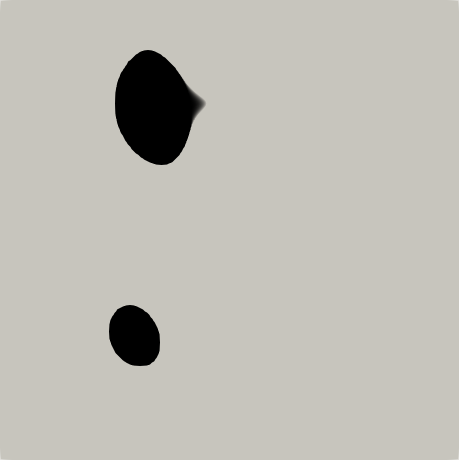
\includegraphics[width=0.35\textwidth]{fixfigs/poll2d-one-set.png}
\end{center}
\caption{Coincidence sets (black) for the 2D bi-obstacle problem in Example \ref{ex:results:advdiff}: $u=0$ (left) and $u=1$ (right).}
\label{fig:results:advdiff}
\end{figure}

For the experiment we used $P_1$ elements, uniform refinement, and a coarse mesh with $m_0=16^d$ nodes so as to minimally-resolve the coincidence set.  The smoother was two (fixed) RS Newton iterations,  with three preconditioned GMRES iterations to approximately solve the step equations.  The additive Schwarz method (ASM) preconditioner applied incomplete factorization (ILU) preconditioning on the blocks.  The coarse solver was RS Newton and LU, iterated to convergence.  Tolerances \id{rtol} $=10^{-5}$, \id{atol} $=10^{-9}$ were used in \eqref{eq:stoppingcriterion}.

F-cycle iteration results are shown in Table \ref{tab:results:advdiff}.  Despite the hint of growing iterations under mesh refinement, a few iterations suffice up to memory-limited resolutions.  For any of the finer mesh runs here, the FASCD F-cycle solver takes less time than generating the $P_1$ mesh hierarchy.
\end{example}

% see git@bitbucket.org:pefarrell/fascd.git: examples/pollutant.py and edplay/results/pollutant.sh|txt
\begin{table}[ht]
\begin{tabular}{lr@{\hskip 7mm}c@{\hskip 4mm}c}
\emph{levels} & $m_J$ & F ($d=2$) & F ($d=3$) \\ \cmidrule{1-4}
 1 &    $16^d$ & 1 & 1 \\
 2 &    $31^d$ & 2 & 2 \\
 3 &    $61^d$ & 2 & 3 \\
 4 &   $121^d$ & 2 & 3 \\
 5 &   $241^d$ & 2 & 4 \\
 6 &   $481^d$ & 2 \\
 7 &   $961^d$ & 3 \\
 8 &  $1921^d$ & 3 \\
 9 &  $3841^d$ & 3
\end{tabular}
\bigskip
\caption{F-cycle iterations for 2D (serial) and 3D (16 processes) solutions of the advection-diffusion bi-obstacle VI problem in Example \ref{ex:results:advdiff}.}
\label{tab:results:advdiff}
\end{table}

\begin{example}   \label{ex:results:sia}
Recall the steady shallow ice approximation (SIA) obstacle problem, Example \ref{ex:sia}, in which the surface elevation $s$ is constrained to exceed the bedrock elevation $b$.  For a test case we set $\Omega=(0,L)^2$, with $L=1800$ km, a radial surface mass balance $a$ function \cite[equation (5.122)]{GreveBlatter2009}, and bumpy, synthetic values for $b\in C^1(\Omega)$, with an elevation range of $1800$ m.  The numerical solution, colored by the ice flow, is shown in Figure \ref{fig:results:siascene}; this used the surface value of the SIA solution, namely $\mathbf{u} = (n+1)(n+2)^{-1} \Gamma (s-b)^{n+1} |\grad s|^{n-1} \grad s$.  As noted in Example \ref{ex:sia} and seen in this Figure, $|\grad s|$ is unbounded at the free boundary, so the solution has low regularity.

\vspace{-2mm}
% to regenerate:
%   $ mpiexec -n 16 --map-by core --bind-to hwthread python3 sia.py -levs 8 -bumps \
%       -mcoarse 8 -fascd_cycle_type full -fascd_monitor -fascd_rtol 2.0e-4 \
%       -fascd_atol 1.0e-8 -o sialev8.pvd
\begin{figure}[ht]
\begin{center}
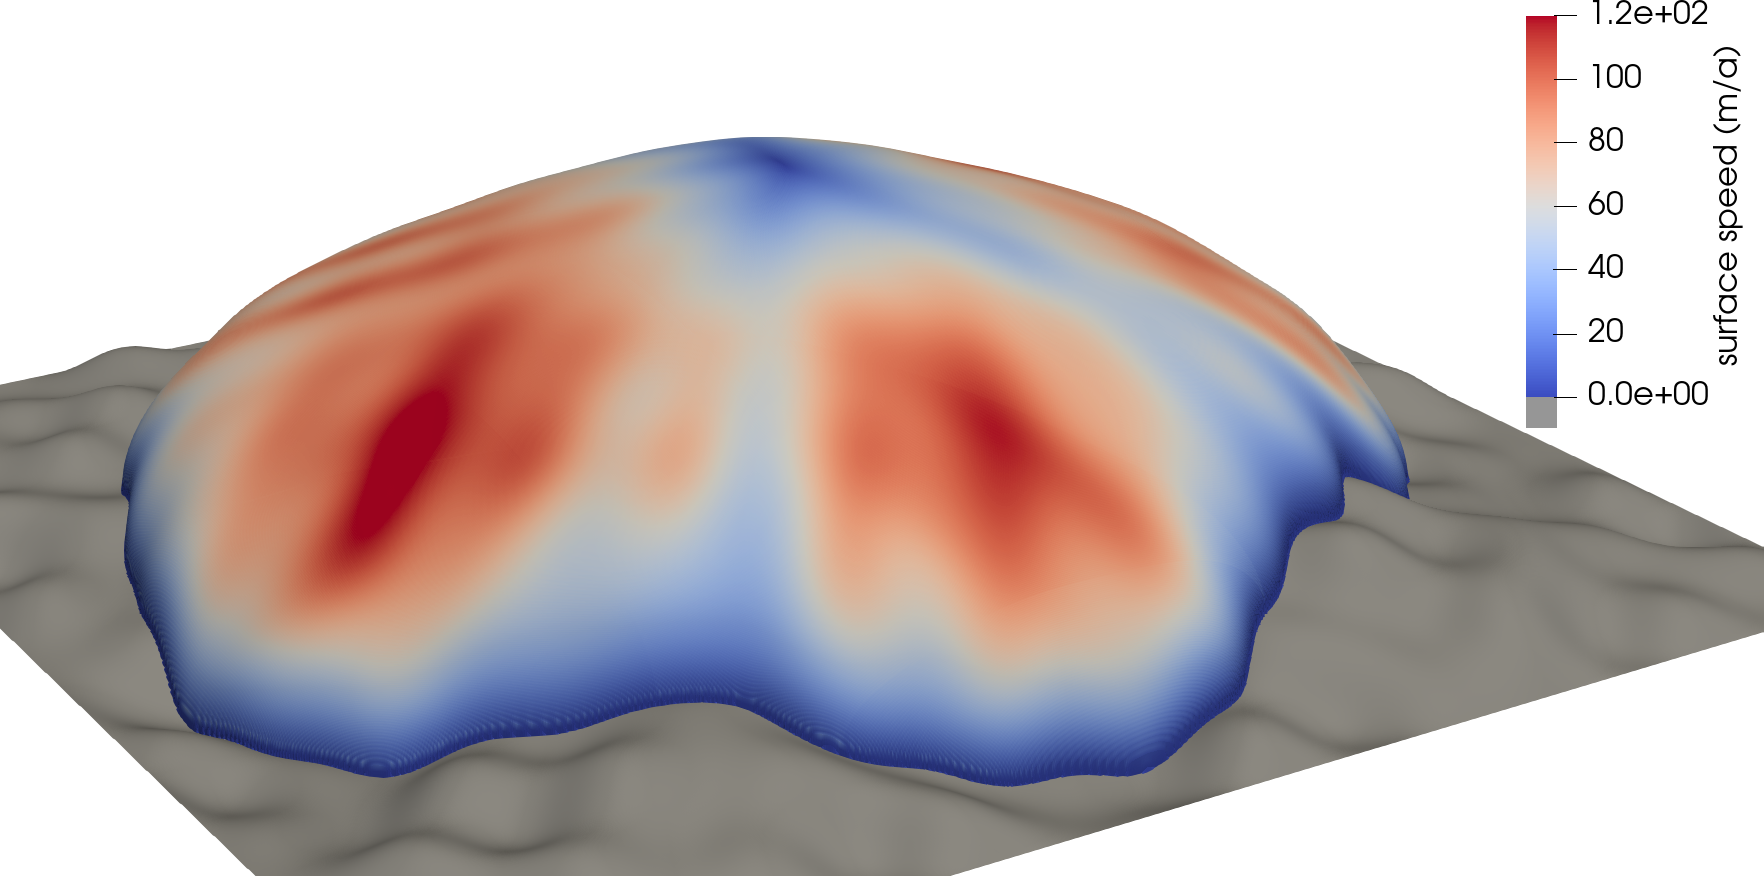
\includegraphics[width=0.95\textwidth]{fixfigs/sialev8scene.png}
\end{center}
\caption{A high-resolution ($m^J\approx 10^6$) solution of Example \ref{ex:sia} over a bumpy bedrock topography, with the ice speed as the surface coloring.}
\label{fig:results:siascene}
\end{figure}

We applied FASCD F-cycles using a smoother of four (fixed) iterations of RS Newton (Section \ref{sec:implementation}), with quadratic backtracking line search.  The step equations were approximately solved, in parallel, by three (fixed) iterations of additive-Schwarz preconditioned GMRES, with ILU preconditioning on the blocks.  The coarse solver was again RS Newton, with LU preconditioning redundantly over all processors.  The coarse mesh was relatively fine, with $m_0=289$ nodes and 512 triangles.  Because of the low regularity of the solution we used \id{rtol} $= 2 \times 10^{-4}$ and \id{atol} $= 10^{-8}$ in \eqref{eq:stoppingcriterion}.  The initial iterate was zero ice: $s=b$.

These solver parameters generate a weak-scaling solver.  For $P$ process solutions we fixed the number of degrees of freedom per process at $m_J/P=1025^2$ and solved over $P=1,4,16$ processes.\footnote{Runs were on a single-node workstation with two Intel Xeon 4210 cpus (2.2GHz), a total of 20 physical cores, and 128 GB shared memory.}  The results in Table \ref{tab:results:siaweak} showing mesh independence in the number of FASCD cycles and clear weak scaling.  The finest mesh result, with $m_J=4097^2=17 \times 10^6$ degrees of freedom, needed under six minutes to solve for the surface elevation of an ice sheet slightly larger than the current Greenland ice sheet ($1.7$ million $\text{km}^2$) at uniform $439$ m resolution.
\end{example}

% see pefarrell-fascd/edplay/siaweak.sh|txt
% time in seconds:
%>> 5*60+[11,36,55]
%ans =      311      336      355
\begin{table}[ht]
\begin{tabular}{c@{\hskip 4mm}c@{\hskip 4mm}c@{\hskip 7mm}c@{\hskip 4mm}c}
P & \emph{levels} & $m_J$ & \emph{F-cycles} & \emph{time} (s) \\ \cmidrule{1-5}
 1 & 7 & $1025^2$ & 4 & 311 \\
 4 & 8 & $2049^2$ & 4 & 336 \\
16 & 9 & $4097^2$ & 4 & 355
\end{tabular}
\bigskip
\caption{Iterations and run time (wall clock, in seconds) for parallel FASCD F-cycle solutions of Example \ref{ex:sia}.}
\label{tab:results:siaweak}
\end{table}


\begin{comment}
from slack, regarding SIA example:
Patrick:  The convergence criteria are relatively loose?
Ed:  Yes, the convergence is loose, and furthermore there is a double-regularization in the nonlinear diffusivity.  The problem is that only the 8/3 power of the solution u is actually in W^{1,p} for p=4; for the flat bed case u^{8/3} is actually C^1.  But the derivative of u itself is not actually integrable, though u is C^0; you can see there is essentially a cliff all the way around the ice sheet.  So as we converge to the exact solution, along the free boundary the P1 elements are trying to match this unbounded derivative, and it struggles at tighter tolerances.  The best (but still not like textbook problems) results are with a Petrov-Galerkin method using Q1, for which the convergence rates are much closer to O(h^2).  See Bueler (2016) for this P-G method, and Jouvet & Bueler (2012) for an existence proof giving u^{8/3} in W^{1,4}.  If you really want to know ...
\end{comment}


\section{Discussion and Conclusion} \label{sec:discussion}

FIXME the observation that up-smoothing is more efficient seems to be new; compare the comments on V(1,0) and V(1,1) cycles in \cite{GraeserKornhuber2009,Tai2003}

FIXME smoother could be AMG

FIXME desired extension to nonlocal variational inequalities


\bibliography{fascd}
\bibliographystyle{siam}


\appendix
\section{Reduction to FAS multigrid for PDEs} \label{app:reductions}

\pr{fascd-vcycle} (Algorithm \ref{alg:fascd}) reduces to the classical FAS multigrid V-cycle for nonlinear PDEs \cite{Trottenbergetal2001}, which itself generalizes linear multigrid, when all inequality constraints are removed.  In fact, suppose we remove the inequality constraints from the finest-level VI problem \eqref{eq:fe:vi} by replacing the finest-level obstacles $\underline{\gamma}^J$ and $\overline{\gamma}^J$ with very negative and positive constants, respectively, thus not constraining the solution $u^J$ or any possible iterate.  The admissible set $\mathcal{K}^J$ of \eqref{eq:fe:vi} is then determined only by the Dirichlet boundary conditions.  Let $\mathcal{V}_0^J \subset \mathcal{V}^J$ denote the linear subspace with zero values on $\partial_D\Omega$.  By replacing the (now) arbitrary element $v-u^J\in\mathcal{V}_0^J$ in \eqref{eq:fe:vi} with ``$v$'' we have the finest-level problem
\begin{equation}
\ip{f^J(u^J)}{v} = \ip{\ell^J}{v} \qquad \text{for all } v\in \mathcal{V}_0^J, \label{eq:app:fas:pde}
\end{equation}
the FE discretization of strong-form PDE $f(u)=\ell$.  The downward $\mathcal{D}^j$ and upward $\mathcal{U}^j$ constraint sets can also be enlarged so that the corrections $y^j$ and $z^j$ in \pr{fascd-vcycle} are never constrained.\footnote{Formally we might do this by choosing constant LDCs with $\underline{\chi}^j \ll 0 \ll \overline{\chi}^j$, but so that ordering property \eqref{eq:fe:chiordering} still holds, and also with large gaps so that $\underline{\phi}^j = \underline{\chi}^j - \underline{\chi}^{j-1} \ll 0 \ll \overline{\phi}^j = \overline{\chi}^j - \overline{\chi}^{j-1}$.}  Thus the corrections $y^j$ and $z^j$ are unconstrained, and lines 2--3 and 5--8 can be removed from Algorithm \ref{alg:fascd}.

Now the downward/upward VIs \eqref{eq:fe:downvi} and \eqref{eq:fe:upvi} are also unconstrained, and can be rewritten as weak forms $\ip{f^j(w^j + y^j)}{v} = \ip{\ell^j}{v}$ and $\ip{f^j(w^j + z^j)}{v} = \ip{\ell^j}{v}$, respectively, for all $v\in \mathcal{V}_0^j$.  Then we combine $u^j=w^j+y^j$, instead of $w^j$ and $y^j$ separately, and similarly $u^j=w^j+z^j$ when up-smoothing.  The smoothers and the coarsest-level solver can be regarded as unconstrained, in-place modifications of $u^j$, so we denote them simply as ``$\text{\pr{smooth}}(\ell^j;u^j)$.''  Noting line 11 of Algorithm \ref{alg:fascd} now says $u^{j-1}=\iR u^j$, after down-smoothing the coarsened source functional computed by line 12 can be rewritten as
\begin{equation}
\ell^{j-1} = f^{j-1}\left(u^{j-1}\right) + R\left(\ell^j-f^j(u^j)\right). \label{eq:app:fas:levelsource}
\end{equation}

Going upward we must be careful that only the coarse correction, and not the coarse solution, is prolonged \cite[remark 5.3.9]{Trottenbergetal2001}.  After up-smoothing on the $j-1$ level the coarse iterate is $u^{j-1}$, but at this point $u^j=w^j + y^j$ contains the result of $j$th-level down-smoothing.  The initial value of the correction $z^j$, before up-smoothing on the $j$th level, is $z^j = y^j + P z^{j-1}$, where $z^{j-1}$ contains the total correction from coarser corrections and $j-1$ level up-smoothing.  Thus the $j$th-level iterate \emph{before} up-smoothing must be set to
    $$w^j + y^j + P z^{j-1} = u^j + P(u^{j-1} - \iR u^j).$$

With these modifications, we have a much-simplified Algorithm \ref{alg:fas}.  This FAS V-cycle appears in various places, for example Algorithm 14 of \cite{Bruneetal2015} or in section 5.3.4 of \cite{Trottenbergetal2001}.

\begin{pseudofloat}[ht]
\begin{pseudo} \label{ps:fas-vcycle}
\pr{fas-vcycle}(\ell^J; u^J)\text{:} \\+
    for $j=J$ downto $j=1$ \\+
      $\text{\pr{smooth}}^{\text{\id{down}}}(\ell^j;u^j)$ \\
      $u^{j-1} = \iR u^j$ \\
      $\ell^{j-1} = f^{j-1}(u^{j-1}) + R \left(\ell^j - f^j(u^j)\right)$ \\-
    $\text{\pr{solve}}(\ell^0;u^0)$ \\
    for $j=1$ to $j=J$ \\+
      $u^j \gets u^j + P (u^{j-1} - \iR u^j)$ \\
      $\text{\pr{smooth}}^{\text{\id{up}}}(\ell^j;u^j)$ \\-
\end{pseudo}
\caption{The standard FAS V-cycle for a discretized PDE $f^J(u^J)=\ell^J$.}
\label{alg:fas}
\end{pseudofloat}


\begin{comment}
%From slack, to not lose

\noindent Patrick : \emph{Interesting that you think Graeser and Kornhuber were barking up the wrong tree.  I still don't quite have my finger on the exact difference in the scheme between GK and the FAS approach. Is there a clean summary somewhere?  (I looked in the mcd-extended manuscript, but couldn't see it in a quick skim.)  Is the difference to GK the monotone multigrid bit, or the particular smoothers used?}

\medskip\noindent
Ed: \cite{GraeserKornhuber2009} only considers the Laplacian lower obstacle case, and they write everything in terms of nonlinear Gauss-Seidel (i.e. optimize one hat function at a time).  They first lay out the \cite{Tai2003} CD strategy as Alg. 4.7, only for V(1,0) cycles.  Then they observe that the convergence rates from \cite{Tai2003} are slower (worse) than if one does "monotone multigrid".  This seems to mean to them that one modifies the coarse hat functions according to whether they overlap the current fine-grid estimate of the coincidence set, "truncated nodal basis functions".  (See the start of \cite{GraeserKornhuber2009} section 5.2.)  I think that making these modifications in Firedrake, so we could try monotone multigrid V-cycles, would be a nightmare.  FASCD does not attempt the monotone multigrid idea at all.

By contrast, FASCD is essentially just the \cite{Tai2003} CD strategy, but (1) without assuming an objective, and (2) with a coarse correction which is FAS in the nonlinear PDE case.  If you apply \cite{Tai2003} CD to a nonquadratic (e.g. p=1.5 p-laplacian) objective then the coarse-grid corrections are optimization problems over the coarse space.  I don't even know how to interpret this in non-optimization VIs?  Or maybe I should say that one can re-interpret this as FAS coarse corrections, and I have done so.

But I have now concluded that everything discussed in \cite{GraeserKornhuber2009} is angels-on-the-head-of-a-pin stuff because the various differences of implementation don't produce any really good multigrid convergence if your smoother is NGS on each level.  I think the convergence proofs in \cite{GraeserKornhuber2009} all depend on this?  There are indeed differences in convergence rates reported in the results at the end of \cite{GraeserKornhuber2009}, but they are all not good compared to how multigrid works on PDEs.  This NGS-based stuff is what I was trying before February, in 1d mostly, with hand-made NGS smoothers, and no Firedrake.

Now, the good thing I was already doing before February was building a version of VI multigrid which makes minimal assumptions on the problem:  FAS (residual need not be linear) and CD (build-up the total V-cycle update in an admissible manner on every level).  Thus it has a chance of working for the ice problems I care about.

As I now see, and can easily demo on the spiral problem in \cite{GraeserKornhuber2009} and on any other classical obstacle problem I have tried, the thing which makes it fly is to realize, as you did, or perhaps as you just take for granted because you are so comfortable with Firedrake, that the smoother can be a grown-up but still O(N) VI solver.  E.g.~a fixed number of iterations of vinewtonrsls+gmres+ilu or whatever.  The role of the FASCD is simply to generate coarse VI problems which, once solved, make helpful admissible additions to the eventual V-cycle update.

So the difference between FASCD and \cite{GraeserKornhuber2009} are: (1) FAS coarse corrections, (2) no attempt to do monotone/truncated multigrid which would be a mess (I think) across the FE infrastructure, (3) clarity on what sets you can use in $V(\nu_1,\nu_2)$ cycles, with bigger up-smoother sets in particular, and most importantly (4) implementation within the mature Firedrake/PETSc library framework where one can easily hook up an active-set Newton step as a smoother.
\end{comment}

\end{document}
